%%%%%%%%%%%%%%%%%% Environment
\documentclass[11pt]{article}
\usepackage[utf8]{inputenc}
%\documentclass{article}
%\usepackage{beamerarticle}

%%%%%%%%%%%%%%%%%% Basic Packages
\usepackage{amsbsy}
\usepackage{amstext}
\usepackage{amsfonts}
\usepackage{amssymb}
\usepackage{amsthm}
\usepackage{amsmath}
\usepackage{bbm}
\usepackage{color}
\usepackage{arydshln}
\usepackage{multirow}
\usepackage{changepage}
\usepackage{threeparttable,booktabs}
\usepackage{enumitem}
\usepackage{subfigure}
\usepackage{natbib}

%\usepackage{natbib}
%\bibliographystyle{abbrvnat}
%\setcitestyle{authoryear,open={((},close={))}}


%%%%%%%%%%%%%%%%%% Style
\usepackage[margin=1in]{geometry}%
\usepackage[doublespacing]{setspace}
%\usepackage{setspace}
%\setstretch{1.618}
%%%%%%%%%%%%%%%%%% Fonts and Graphics
\usepackage[cjk]{kotex} %Korean TeX
\usepackage[pdftex]{graphicx}

%%%%%%%%%%%%%%%%%% Theorem
\newtheorem{Theorem}{Theorem}
\newtheorem{Lemma}{Lemma}
\newtheorem{assumption}{Assumption}
\newtheorem{prop}{Proposition}
\newtheorem{corollary}{Corollary}
\newcommand{\ju}{\textcolor{cyan}}
\newcommand{\yj}{\textcolor{magenta}}
\usepackage{apptools}
\AtAppendix{\counterwithin{Lemma}{section}}
\AtAppendix{\counterwithin{table}{section}}
\AtAppendix{\counterwithin{figure}{section}}

%%%%%%%%%%%%%%%%%% Bibliography and Appendices
%\usepackage[natbibapa]{apacite} % Including URLs in bibliography
\usepackage{natbib}
\usepackage[hyphens]{url} % Including URLs in bibliography
%\usepackage[toc,page,title]{appendix} % Extra control of appendices
\usepackage[titletoc,toc,title]{appendix}
\usepackage{chngcntr}

%%%%%%%%%%%%%%%%%Appendix title
\let\oldappendix\appendix
\makeatletter
\renewcommand{\appendix}{%
  \addtocontents{toc}{\let\protect\numberline\protect\appendixnumberline}%
  \renewcommand{\@seccntformat}[1]{Appendix~\csname the##1\endcsname\quad}%
  \oldappendix
}
\makeatother

%%%%%%%%%%%%%%%%%% Cover Page
\title{
	\onehalfspacing
	{\huge Sharing Economy in the Cloud:\\Pricing Schemes for Peer-to-Peer Storage Platforms}
}
\author{
	YoungJae Jang$^1$
	\and Jaeung Sim$^2$\thanks{Corresponding author. E-mail address: jaeung.sim@uconn.edu}
	\and Kun Soo Park$^3$
	\and Daegon Cho$^4$
}
\date{%
	\onehalfspacing
	$^1$MineIS, Seoul 04798, Republic of Korea\\%
	$^2$University of Connecticut, Stamford, CT 06901, USA\\%
	$^3$Seoul National University, Seoul 08825, Republic of Korea\\%
	$^4$Yonsei University, Seoul 03722, Republic of Korea\\[2ex]%
	\today
}

%%%%%%%%%%%%%%%%%% Font Size of Abstract
\makeatletter
\renewenvironment{abstract}{%
	\if@twocolumn
	\section*{\abstractname}%
	\else %% <- here I've removed \small
	\begin{center}%
		{\bfseries \large\abstractname\vspace{\z@}}%  %% <- here I've added \Large
	\end{center}%
	\quotation
	\fi}
{\if@twocolumn\else\endquotation\fi}
\makeatother

%%%%%%%%%%%%%%%%%% Beginning of the Manuscript
\begin{document}
%
%\begin{center}{\LARGE Sharing Economy in the Cloud:\\
%Pricing Schemes for Peer-to-Peer Storage Platforms}\end{center}
%
\begin{center}{\LARGE \textbf{Sharing Economy in the Cloud:\\
Pricing Schemes for Peer-to-Peer Storage Platforms}}\end{center}
%\maketitle
%
%
\begin{abstract}
%	\onehalfspacing
\setlength{\baselineskip}{15pt}
	\noindent
	% Each submitted article must contain a structured abstract (no more than 300 words) that is based on the following subsections (without technical jargon):
    % Problem definition: What is your research problem?
    % Methodology/results: What is the research method and the key findings?
    % Managerial implications: How can academics / managers / decision makers benefit from your paper?
    % Please include the above three sections in your abstract followed by the appropriate information in both Step 1 of the submission process and in the main paper file.
	{\normalsize
	% 2024-10-14 version (190 words)
    \textbf{\textit{Problem definition:}} With rising data storage demands, peer-to-peer (P2P) storage platforms using blockchain have emerged as viable alternatives to traditional cloud services. Although blockchain supports secure crowdsourcing of unused storage, P2P platforms struggle to ensure consistent storage availability. Incentive schemes encourage participation, yet the effectiveness of various pricing models is under-researched. This paper examines the impacts of three pricing schemes—two-part tariff, subscription, and hybrid—on P2P platforms' short-term profits and overall system welfare. \textbf{\textit{Methodology/results:}} Using a game-theoretic model, we analyze interactions among renters, providers, and the platform. We find that the two-part tariff maximizes short-term profits, while subscription pricing yields the highest renter surplus. For total welfare, the optimal scheme depends on provider availability: subscription pricing maximizes welfare when providers are abundant, whereas hybrid or two-part tariff pricing optimizes welfare in cases of provider scarcity. \textbf{\textit{Managerial implications:}} These insights offer strategic guidance for P2P storage platforms. Given the early stage of this market, platforms may benefit from prioritizing total surplus over short-term profits to expand their user base. However, if attracting providers is more challenging than attracting renters, platforms might need to adopt higher-cost schemes to compensate for bandwidth provision adequately.}
\end{abstract}
\baselineskip 15.5pt
\hspace{0.2cm} {\sc Keywords:} Cloud computing; peer-to-peer markets; pricing schemes; sharing economy
%
%
%\clearpage

%\linespread{5}
%\onehalfspacing
\setlength{\baselineskip}{15pt}
\doublespacing
%
%
\section{Introduction}\label{sec:intro}
Despite the rapid growth of public cloud services like Amazon Web Services (AWS), the storage supply is projected to fall short of meeting the surging data demands. According to the International Data Corporation (IDC), global spare storage capacity in the commercial market decreased from 33\% in 2018 to an expected 15\% in 2020 \citep{robb2015space, idc2018worldwide}. One potential solution to this impending shortage is utilizing the unused storage space on billions of personal computers (PCs), estimated at 250 exabytes globally, surpassing the combined capacity of all public cloud services \citep{thompson2014cloud}. By enabling individuals to share this underutilized space, peer-to-peer (P2P) storage could complement and compete with conventional cloud services. However, P2P storage between PCs has not gained widespread adoption due to privacy and security concerns.

To address these challenges, new decentralized P2P storage platforms utilizing cloud computing and blockchain technology have emerged, offering enhanced data encryption and security \citep{protocol2017filecoin, vorick2014sia, wilkinson2016storj}. These platforms fragment large files and distribute them across multiple providers, ensuring no single provider can access the complete file. Blockchain technology further ensures secure, verifiable storage contracts between renters and providers, with incentives to maintain system stability.

Although still in its early stages, P2P storage has gained significant traction in the cryptocurrency market with massive successes from the initial coin offerings (ICOs). For instance, Storj, a platform that appeared in 2014, has already reached a market capitalization of \$391.0 million with a total storage capacity of 36.7 PB, 71,689 platform users, and 285 million files. Similarly, Sia has reached a market capitalization of \$872.9 million. It has a total 3.5PB storage capacity and 1.2 million accumulated downloads. Filecoin, which appeared relatively recently, set a new record in ICO funding of \$257 million in 2017 and currently ranks 24th among all cryptocurrencies with a market capitalization of \$6.816 billion. Surprisingly, it reached a total of 629.3PB storage capacity within ten months of its launch. This growth highlights the potential of blockchain-enabled P2P storage to overcome security issues and scale rapidly.\footnote{Please refer to recent statistics of Storj, Sia, and Filecoin from https://www.storj.io/, https://siastats.info/, and https://file.app/, respectively. All statistics in this paragraph were observed on August 12, 2021.} 

However, P2P platforms face challenges related to storage availability and service reliability, as they cannot directly control storage capacity or provider availability. To mitigate this, they rely on economic incentives to attract and retain providers \citep{babich2020distributed, beck2018governance}. These platforms typically charge renters a storage fee and a bandwidth fee for file access. For example, Sia and Storj use two-part tariffs, combining storage and bandwidth fees, while Storj recently introduced a pricing scheme with free usage up to a threshold.\footnote{Storj's latest pricing policy is available at https://www.storj.io/pricing.} In spite of the importance of pricing schemes for attracting participants, little is known about their impact on the platform, providers, and renters.

Thus motivated, this study aims to investigate a P2P storage platform's optimal design of service fees, storage redundancy algorithms, and the implications of pricing schemes on profit and surplus. We incorporate pricing schemes that either centralized public cloud services or P2P storage platforms have adopted in practice. Specifically, P2P storage platforms have widely adopted the two-part tariff, while conventional public cloud services have widely used the pay-per-use, subscription-based, and hybrid pricing \citep{kansal2014pricing}. We analyze how these schemes affect providers, renters, and the platform's outcomes in this emerging market.

We consider three pricing schemes: First, the two-part tariff, which combines a lump-sum fee for storage with a pay-per-use fee for download bandwidth. Second, subscription-based pricing, where renters pay for storage capacity and receive unlimited access to stored files. Finally, hybrid pricing, which includes a lump-sum storage fee and a limited free bandwidth allowance, with pay-per-use charges for excess downloads. We analyze the effects of these schemes on P2P storage services, addressing the following research questions: \textit{How should the platform determine its redundancy algorithm and service fees under each pricing scheme? Which scheme maximizes the platform's profit and overall system surplus? How do the numbers of potential renters and providers impact the effectiveness of pricing schemes?}

To answer these questions, we develop a game-theoretic model of a profit-seeking P2P storage platform mediating between providers and renters. The platform sets its redundancy algorithm and service fees based on the given pricing scheme. Providers with heterogeneous operational costs decide whether to participate and share storage, while renters with a varying willingness to pay choose whether to adopt the platform. The platform earns commissions from transactions, and providers' costs increase with bandwidth usage. The platform uses a $k$-of-$m$ erasure coding scheme, where files are divided into $k$ fragments and distributed across $m$ providers. The redundancy rate, $m/k$, limits storage availability based on provider capacity.

Our results suggest that the platform should set the redundancy algorithms to minimize the total providers' operating costs for all pricing schemes. We also show that when the first-best prices---which maximizes the platform's profit when the size of potential providers is sufficient---are applicable, the two-part tariff always maximizes the platform's profit and provider surplus, and hybrid pricing follows. Notably, hybrid pricing yields the same outcomes when it offers a small amount of free download volume. Regarding the renter surplus, subscription-based pricing is most effective because the gain of renters with a higher usage frequency exceeds the loss from renters leaving the service due to a high storage fee. Consequently, subscription-based pricing outperforms other pricing schemes in terms of total surplus.

Markedly, we find that the impacts of pricing schemes significantly differ when potential providers are relatively scarce. If the size of potential providers is insufficient to fulfill the storage demand, the platform's optimal fees are subject to the market-clearing prices---which makes supply and demand equivalent---instead of the first-best prices. In this situation, subscription-based pricing does not necessarily generate the maximum total surplus. In other words, the two-part tariff and the hybrid pricing can dominate the subscription-based pricing concerning the platform's profit and the total surplus. 

We further validate our findings by examining how endogenous commission rates affect the results. We find that our main insights continue to hold when the platform determines commission rates endogenously, although the thresholds that enable the first-best prices change accordingly.

\section{Related Literature}\label{sec:literature}

\subsection{Pricing and Capacity Management in Centralized Cloud}
Extensive research has explored pricing schemes in centralized services. For example, \citet{randhawa2008usage} studied a rental firm's choice between a subscription model with limited simultaneous rentals and a pay-per-use model without restrictions, finding that subscriptions increase social welfare and consumer surplus. Similarly, \citet{cachon2011pricing} compared subscription and pay-per-use pricing in a queuing model, showing that subscription pricing is generally more profitable, especially when customer service rates are diverse.

In centralized cloud platforms, pricing strategies and capacity management have also received attention \citep{fazli2018effects, chen2019pricing, chen2021discount, li2018should, kansal2014pricing, arbabian2021capacity}. For instance, \citet{chen2019pricing} analyzed reservation-based and utilization-based pricing in cloud platforms, discovering that customers with low demand volatility prefer reservation-based pricing, while those with high volatility opt for utilization-based pricing. Likewise, \citet{nunez2021leveraging} proposed hybrid pricing for Infrastructure as a Service (IaaS) cloud services to manage slack capacity by combining contract and on-demand services under varying market conditions.

While centralized platforms have been extensively studied, little work has addressed pricing and capacity management in P2P cloud platforms, where pricing simultaneously affects service demand and provider supply. This two-sided aspect is crucial, as it influences both the availability and utilization of services on P2P platforms, making pricing schemes integral to understanding capacity management in decentralized environments.

\subsection{P2P Sharing of Computing Resources}
This paper is also related to the literature on sharing platforms for computing resources. The vast majority of studies in this stream focused on the mechanism design of P2P file-sharing networks \citep{antoniadis2004p2p, casadesus2010p2p, de2017quality, ghasemkhani2018contracting, golle2001incentives}. For instance, \citet{antoniadis2004p2p} conducted a numerical analysis to compare several incentive schemes and suggested that a simple fixed fee scheme, where all peers are required to share a standard number of files, can achieve a high level of network efficiency. 

\citet{de2017quality} studied how individual peers make sharing decisions under quality-of-service based pricing schemes. They showed that socially optimal behaviors are induced where a pricing scheme does not charge users for content requests, while profit maximization is achieved where a pricing scheme charges users for requesting content. \citet{ghasemkhani2018contracting} proposed a contracting scheme for a monopolistic P2P file-sharing network, in which the network compensates each contracted peer node for the supply of files. They investigated the optimal reward scheme for the profit-seeking P2P network regarding network structures, content availability, propagation delay, among others.

It is worth noting that this literature stream has concentrated on file-sharing platforms only. Although a variety of computing resources---such as storage capacity, CPU power, and internet bandwidth---have recently been shared in online markets \citep{dickson2019monetizing, sharma2020blockchain}, we are aware of no study that examined sharing platforms for these resources.
 
\subsection{Sharing Economy and Online Platforms}
Several studies highlight the benefits of sharing idle resources through platforms like Airbnb and Uber. For instance, \citet{zervas2017rise} found that Airbnb's entry lowered hotel prices, benefiting consumers, while \citet{lee2018battle} showed that Uber reduces search costs for riders. Although many studies affirm the consumer benefits of these platforms \citep{einav2016peer, greenwood2017show}, some analytical work cautions that they may raise long-term prices or lead to consumer discrimination \citep{abhishek2021business, jiang2018collaborative, weber2016product}. \citet{tian2018effects} found that sharing platforms can increase a retailer's gross profit margin in distribution channels.

Theoretical frameworks for pricing strategies on sharing platforms have also emerged \citep{bai2019coordinating, benjaafar2019peer, cachon2017role, bimpikis2019spatial, taylor2018demand}. \citet{benjaafar2019peer} compared profit-maximizing and welfare-maximizing platforms, finding modest differences in social welfare outcomes. \citet{cachon2017role} analyzed pricing schemes, including surge pricing, in platforms with self-scheduling providers, revealing that surge pricing nearly maximizes profit and benefits both providers and consumers when labor costs are high. Recently, \citet{zhang2022two} explored the effects of wage schemes, such as fixed and dynamic commission rates, on competition between platforms, showing that the choice of scheme depends on the relative competitiveness of supply and demand, impacting profits and surpluses for all parties.

\subsection{Contributions to the Literature}
Our study provides a foundational theoretical framework for pricing in decentralized cloud platforms. Unlike centralized cloud services, P2P cloud platforms depend on independent providers with varying storage capacities, meaning pricing decisions impact both service levels and costs for customers. Our model incorporates providers' participation decisions, renters' adoption choices, and the interactions between these groups to address this unique complexity.

We also explore subscription-based pricing, a common strategy in public cloud services \citep{kansal2014pricing}, but not yet widely implemented in P2P storage. We show that pricing schemes' effects on system surplus vary with the number of providers relative to storage demand. When provider numbers are sufficient, subscription-based pricing maximizes both renter and system surplus. However, with limited providers, two-part tariffs or hybrid pricing can surpass subscription-based models in terms of platform profit and total surplus.

Our framework includes the platform's algorithmic decision-making, specifically focusing on redundancy algorithms that minimize total provider operating costs, regardless of the pricing scheme. This separation suggests that P2P platforms can optimize pricing strategies and redundancy algorithms independently, enhancing overall efficiency without entangling these key decisions.

Lastly, our study extends insights on pricing for sharing platforms across computing resources such as storage, CPU power, and bandwidth \citep{dickson2019monetizing, sharma2020blockchain}. Unlike simple file-sharing, P2P storage services require both storage and subsequent bandwidth fees, making the two-part tariff, with separate storage and bandwidth charges, highly relevant. By considering provider cost heterogeneity and renter usage impacts, our model offers a robust framework for addressing pricing and service decisions, relevant for a broader sharing economy and extending prior research on pricing strategies in multi-sided platforms like ride-sharing and delivery services \citep{cachon2017role, zhang2022two}.

\section{Model}\label{sec:model}

In this section, we first describe our model setups and players, which is followed by the key decisions of players. We present the summary of basic notations in Table \ref{tbl:summary}. The proofs of all lemmas and theorems appear in Online Appendix \ref{app:proof}.

\begin{table}[h] \centering
\textbf{\caption{A Summary of Basic Notations}\label{tbl:summary}}
\vspace{0.1in}
\begin{tabular}{l  p{14cm}}
\toprule
\textbf{Notation} & \textbf{Description} \\\hline
\multicolumn{2}{l}{\textbf{Parameters: Environment}}\\\hline
$n_r$ & Number of potential renters \\
$n_p$ & Number of potential providers \\
$\alpha$ & Proportion of revenue that providers receive \\\hline
\multicolumn{2}{l}{\textbf{Parameters: Heterogeneity}}\\\hline
$u_i$ & Renter $i$'s unit utility of bandwidth usage \\
$\lambda_i$ & Renter $i$'s bandwidth usage \\
$\rho_j$ & Provider $j$'s sensitivity to bandwidth provision\\\hline
\multicolumn{2}{l}{\textbf{Platform's decision variables}}\\\hline
$\theta$ & (Algorithm decision) Redundancy rate \\
$t$ & (Algorithm decision) Required uptime, determining unit operating cost $\xi$\\
$p_s$ & (Pricing decision) Storage fee\\
$p_b$ & (Pricing decision) Bandwidth fee\\\hline
\multicolumn{2}{l}{\textbf{Performance measures}}\\\hline
$\Pi$ & Platform's profit\\
TS & Total system surplus\\
\bottomrule
\end{tabular}
\end{table}

\subsection{Model Setups}\label{subsec:setups}

We consider a P2P storage platform where some peers provide their unused storage (\textit{providers}) and others rent the storage space and request downloading of stored files (\textit{renters}). The platform offers two services to renters: \textit{i)} the initial file storage (the storage service), and \textit{ii)} access to the stored files via a download request (the bandwidth service). Upon a storage request, the platform splits a renter's file into $k$ fragments, assigning them to $m$ ($> k$) providers.\footnote{P2P storage platforms employ a $k$-of-$m$ erasure coding scheme, under which an original file is divided into $k$ shards, and the shards are re-coded into $m$ encrypted fragments ($m > k$) \citep{wilkinson2016storj}. Since any $k$ fragments among $m$ fragments are sufficient to reconstruct the file, erasure coding enables high reliability with low expansion factors \citep{weatherspoon2002erasure}. See Online Appendix \ref{app:algorithm} for technical details.} After completing the initial file storage, a renter can request a download of the stored file to the providers.

Since the availability of stored files to storage renters is critical for P2P storage services, the P2P storage platforms should maintain the likelihood of file transfer failure negligible. Therefore, the platform needs to carefully set the algorithmic parameters: 1) the redundancy in the erasure coding $\theta \equiv \frac{m}{k}$, which measures data duplication, and 2) uptime $t$, representing providers' connection time to the network \citep{protocol2017filecoin, vorick2014sia, wilkinson2016storj}. We postulate that the platform considers the algorithm parameter combinations that maintain the same failure probability. In doing so, the platform may increase $\theta$ and decrease $t$ or vice versa. When the platform decides to raise $\theta$ and correspondingly reduce $t$, participating renters have to pay higher storage costs due to the higher redundancy rate, while providers can mitigate their operating burden. Consequently, the P2P network imposes a higher burden on renters. On the other hand, when the platform meets the probability by increasing $t$ rather than $\theta$, providers have to bear higher operating costs due to higher bandwidth uptime.

P2P storage platforms aim to achieve near-zero failure probabilities with these. Theoretically and practically, it has shown to be extremely rare for well-performing P2P networks to experience file transfer failure.\footnote{For instance, the failure probability of a $k$-of-$m$ erasure coding is 5.266e-10 where $k=6$, $m=18$, and $t=0.90$ \citep{wilkinson2016storj}. In Sia's storage network, providers must maintain a 95–98\% uptime, enabling the network to achieve 99.9999\% availability of stored files to renters. Online Appendix \ref{app:algorithm} provides more details on the algorithmic backgrounds.} Thus, we assume that the platform targets an availability goal near 100\%, only considering the $(\theta, t)$ combinations that meet this goal, thus excluding file transfer failure probability from our model.

\begin{figure}[ht!]
\centering
\includegraphics[width=14cm]{fig1_timeline_minor_revision.pdf} 
\textbf{\caption{The Sequence of Events}\label{fig:timeline}}
\end{figure}

Figure \ref{fig:timeline} illustrates the sequence of the events for the platform, providers, and renters in our model. Initially, the platform observes the potential market size of peers ($n_r$ and $n_p$). Given the \textit{exogenous} market condition, pricing scheme, and commission rate, the platform first determines its redundancy algorithm ($\theta$, $t$), and then, it decides its service fees $(p_s, p_b)$ based on this setup. This is consistent with the current market situation, where the development of a redundancy algorithm takes several months or years.\footnote{Sia and Storj have not officially changed their algorithms since their releases. Also, Sia has not adopted the 64-of-96 algorithm, which this platform announced its development plan in 2020. The announcement is available at https://blog.sia.tech/cloud-storage-for-2-tb-mo-8a34043e93bb.} Subsequently, potential
providers decide whether to join based on expected profits. Once onboard, providers offer unused storage to renters. Lastly, potential renters assess the service fees and storage availability, determining whether to adopt the service. Once the P2P storage service is adopted, a renter starts using the storage spaces provided by the providers.

We now further explain three essential players in the P2P file-sharing service: renters, providers, and a service platform.

\textbf{\textit{Renters.}} We consider a renter requiring storage for a unit volume of files, with a total potential renter pool of $n_r$. Each potential renter decides whether to adopt the P2P storage platform and rent the storage space from providers. The renters will join the platform if their usage value exceeds total service costs. In this model, renters vary in bandwidth usage, denoted by $\lambda$, representing download frequency. Consistent with cloud-resource usage patterns showing heavy tails compared with exponential, log-normal, and normal distributions \citep{loboz2012cloud}, similarly to other digital resources like smartphone and YouTube usage \citep{falaki2010div, gill2008char}, we assume that a renter's bandwidth usage $\lambda$ follows the Pareto distribution in keeping with the extant literature \citep{bandi2015robust, li2018should, ramirez2017adapt}.

Based on this assumption, the probability distribution function of the bandwidth usage level can be expressed as $f(\lambda) = \frac{b \lambda_0^b}{\lambda^{b+1}}$, where the minimum bandwidth usage level is denoted by $\lambda_0$. For analytical tractability, we simplify our assumption such that the distribution of bandwidth usage level is characterized by the parameter value of $b = 2$. To incorporate heterogeneous valuation, we assume that renter $i$'s utility per unit volume of bandwidth usage, $u_i$, follows a uniform distribution $u_i \sim U[0, 1]$. As a result, renter $i$'s total utility is $\lambda_i u_i$. To focus on the interplay among the platform, providers, and renters, we assume that $\lambda_i$ and $u_i$ are independent. The total service cost for storage and bandwidth, $c(p_s, p_b, \lambda_i)$, depends on the platform's fees ($p_s, p_b$) and usage level $\lambda$. Since bandwidth utility $u_i$ is bounded between $0$ and $1$, we limit the platform's bandwidth fee to $p_b \le 1$ to ensure positive utility for all renters.

\textbf{\textit{Providers.}} We consider $n_p$ potential providers, each with a unit of unused storage. A provider will participate in the P2P storage platform if expected revenue exceeds operating costs, earning from storage and bandwidth services after platform commissions. Let $\alpha \in [0, 1]$ denote the provider's share of service fees from renters. Storage revenue is proportional to $\alpha p_s$ across pricing schemes, while bandwidth revenue varies with the scheme.

We incorporate heterogeneous operating costs of providers for sharing each provider's unit volume of unused space. The operating costs include factors like resource opportunity cost, device obsolescence, and Internet and electricity costs. These costs, which increase with download requests and uptime, are represented as $\rho_j \hat{\omega}_b \xi$, where $\rho_j$ reflects provider $j$'s sensitivity to bandwidth provision, following a uniform distribution $U[0,1]$. Here, $\hat{\omega}_b$ is the expected bandwidth per provider,\footnote{We denote the total bandwidth volume of all participating providers by $\omega_b$.} and $\xi(t)$ is the unit operating cost, which rises with uptime $t$ (hereafter simplified as $\xi$).

Also, we only consider the case where operating costs are non-negligible in a provider's in-out decision. Specifically, when $\xi$ is substantially small, the platform makes all potential providers join the network for all pricing schemes, preventing us from exploring the interplay between providers' and renters' decisions. Considering that the profitability and operating costs are major concerns in online forums for P2P storage platforms, such conditions are unrealistic in practice.\footnote{The profitability and operating costs are widely discussed among Storj's official forum (https://forum.storj.io/) and other forum users (e.g., Reddit).} Therefore, we assume that $\xi$ is sufficiently large; technically, $\xi > \frac{3}{4}\alpha$.

\textbf{\textit{Platform.}} We consider a profit-seeking P2P storage platform that connects renters and providers, enabling encrypted storage contracts between them. The platform first sets the redundancy rate $\theta$ and required uptime $t$, allowing renters to use provider storage until demand times $\theta$ equals total capacity. The platform then sets service fees $p_s$ and $p_b$ based on market conditions, earning profits by charging a commission on completed transactions. For example, Sia operates with $\theta=3$ and $t=0.98$, charging a 3.9\% commission on storage contract payouts. We assume an exogenously set commission rate ($1-\alpha$) to focus on pricing scheme characteristics in Sections \ref{sec:analysis1} and \ref{sec:analysis2} and relax this assumption to consider endogenous commission rates in Section \ref{sec:analysis3}.

Service availability depends on both the storage provided and requested, and the redundancy rate $\theta$ impacts availability by reducing the available space to renters. Thus, the platform's capacity depends on whether the market's potential provider capacity, divided by $\theta$ (i.e., $n_p/\theta$), meets or exceeds demand ($n_r$). We consider two scenarios: 1) the case of a sufficient base of potential providers in the market, and 2) the case of an insufficient base of potential providers.

\subsection{Peer Decisions}\label{subsec:peers}
We describe peer decisions under a given platform's decision. Table \ref{tbl:volume} presents the summary of notations for intermediate variables, including volume variables and peer utility.

\begin{table}[h] \small \centering
\textbf{\caption{A Summary of Intermediate Variable Notations}\label{tbl:volume}}
\vspace{0.1in}
\begin{tabular}{c  c  c  p{10cm}}
\toprule
\textbf{Notation}  & \textbf{Peer} & \textbf{Unit}& \textbf{Description} \\ \hline
\multicolumn{4}{l}{\textbf{Volume notation}}\\ \hline
$\upsilon_s$ &\multirow{2}{*}{Renter}&\multirow{4}{*}{Total}& Total storage volume of renters willing to adopt the platform\\
$\upsilon_b$&&& Total bandwidth volume of renters willing to adopt the platform \\\cline{2-2}
$\omega_s$ &\multirow{4}{*}{Provider}&& Total storage volume of providers willing to join the platform\\
$\omega_b$  &&& Total bandwidth volume of providers willing to join the platform \\\cline{3-3}
$\hat{\omega}_s$&&\multirow{2}{*}{Individual}& Expected storage volume for each provider\\
$\hat{\omega}_b$ &&& Expected bandwidth volume for each provider\\\midrule
\multicolumn{4}{l}{\textbf{Peer utility}}\\\hline
$U_i$ & Renter & \multirow{2}{*}{Individual}& Renter $i$'s total utility\\\cline{2-2}
$\pi_j$&Provider&& Provider $j$'s profit\\
\bottomrule
\end{tabular}
\begin{tablenotes}
  \small
  \item Note. The following equations hold: $\upsilon_b = \upsilon_{bp} + \upsilon_{bf}$, $\omega_b = \omega_{bp} + \omega_{bf}$, $\hat{\omega}_b = \hat{\omega}_{bp} + \hat{\omega}_{bf}$, where the subscripts \textit{bp} and \textit{bf} indicate the paid bandwidth volume and the free (i.e., unpaid) bandwidth volume, respectively. 
\end{tablenotes}
\end{table}

\subsubsection{A Renter's Decision} Renter $i$ decides to adopt the P2P storage service if the expected utility $U_i = \lambda_i u_i - c(p_s, p_b, \lambda_i)$ is higher than or equal to zero, where $c(p_s, p_b, \lambda_i)$ indicates the total service cost. Since a renter's service cost structure differs across pricing schemes, we provide the total storage and bandwidth volumes for each scheme. For simplicity, we denote the two-part tariff, subscription-based pricing, and hybrid pricing by superscripts $T$, $S$, and $H$, respectively.
 
\textbf{\textit{Two-part Tariff.}} In this pricing scheme, the platform charges renters a lump-sum storage fee of $p_s$ for storage and a pay-per-use bandwidth fee of $p_b$ for each unit request for download. The total service cost for renter $i$ is $c(p_s, p_b, \lambda_i) = \theta p_s + \lambda_i p_b$, where $\theta p_s$ represents the storage cost (adjusted by redundancy rate $\theta$), and $\lambda_i p_b$ covers the bandwidth cost based on usage $\lambda_i$. Thus, the utility for renter $i$ is $U_i = \lambda_i u_i - \theta p_s - \lambda_i p_b$.

We define $u^T(\lambda) \equiv \frac{\theta p_s}{\lambda} + p_b$, which indicates the lower bound of $u_i$ for renters who adopt the service with given bandwidth usage level $\lambda$ in the two-part tariff. Then, renter $i$ would adopt the platform if and only if $u_i \ge u^T(\lambda)$. Considering the distribution function of renters' bandwidth usage levels $\lambda$, we obtain the total expected storage demand and bandwidth demand from renters in the two-part tariff, denoted by $\upsilon_s^T$ and $\upsilon_b^T$, as:
\begin{equation*}
\begin{aligned}
&\upsilon_s^T = \int_{\max\{\lambda_0, \lambda^T\}}^{\infty} \{1-u^T(\lambda)\} f(\lambda) d \lambda,\\
&\upsilon_{b}^T = \int_{\max\{\lambda_0, \lambda^T\}}^{\infty} \{1-u^T(\lambda)\} \lambda f(\lambda) d \lambda \; (=\upsilon_{bp}^T),\\
&\text{where } \lambda^T = \frac{\theta p_s}{1-p_b}.
%&\upsilon_{bf}^T = 0\\
\end{aligned}
\end{equation*}

We also note that the free download volume of the bandwidth service $\upsilon_{bf}^T$ is zero because the platform does not offer the free bandwidth allowance in the two-part tariff.

\textbf{\textit{Subscription-based Pricing.}} This pricing scheme charges only a lump-sum fee for the storage service and offers the bandwidth service for free. Therefore, regardless of service usage level $\lambda$, renter $i$'s total service cost only consists of the storage fee multiplied by the redundancy rate (i.e., $c(p_s, p_b, \lambda_i) = \theta p_s$). Then, renter $i$'s utility is expressed as $U_i = \lambda_i u_i - \theta p_s$. Similarly to $u^T(\lambda)$, we define $u^S(\lambda) = \frac{\theta p_s }{\lambda}$ as the lowest $u_i$ of renters adopting the service for a given bandwidth usage level $\lambda$ in subscription-based pricing. The expected total storage demand and bandwidth demand from renters with respect to renters' $\lambda$, which is denoted by $\upsilon_s^S$ and $\upsilon_b^S$ is expressed as:
\begin{equation*}
\begin{aligned}
&\upsilon_s^S = \int_{\max\{\lambda_0, \lambda^S\}}^{\infty} \{1-u^S(\lambda)\} f(\lambda) d \lambda, \\
&\upsilon_{b}^S = \int_{\max\{\lambda_0, \lambda^S\}}^{\infty} \{1-u^S(\lambda)\} \lambda f(\lambda) d \lambda \; (=\upsilon_{bf}^S),\\
%&\upsilon_{bp}^S = 0\\
&\text{where } \lambda^S = \theta p_s.
\end{aligned}
\end{equation*}
Since the platform does not charge renters bandwidth fees, providers are not compensated for offering the bandwidth service. Accordingly, we have $\upsilon_{bp}^S = 0$.

\textbf{\textit{Hybrid Pricing.}} This pricing scheme includes both the storage fee $p_s$ and a limited free bandwidth up to $q \lambda_0$, where $\lambda_0$ represents the minimum bandwidth usage level among all potential renters, and $q\, (\ge 0)$ refers to a coefficient of the free bandwidth allowance. Note that $q = 0$ makes hybrid pricing equivalent to the two-part tariff. The platform charges the bandwidth fee $p_b$ for the bandwidth usage that exceeds $q \lambda_0$. Therefore, renter $i$'s service cost is calculated as $c(p_s, p_b, \lambda_i) = \theta p_s + \max\{\lambda_i - q \lambda_0, 0\} p_b$, and her utility is $U_i = \lambda_i u_i - \theta p_s - \max\{\lambda_i - q \lambda_0, 0\} p_b$. For hybrid pricing, we define $u^H(\lambda) \equiv \frac{\theta p_s +\max\{\lambda - q \lambda_0, 0\} p_b}{\lambda}$ as the lowest $u_i$ among renters who have a bandwidth usage level $\lambda$ and adopt the P2P storage service.

The characteristics of hybrid pricing vary significantly based on the free bandwidth amount $q \lambda_0$. We denote hybrid pricing with $0 \le q \le 1$ and $q \ge 1$ by superscripts $Hl$ and $Hh$, respectively. When $0 \le q \le 1$, all adopting renters have bandwidth usage above $q \lambda_0$, so each renter pays for the bandwidth used beyond the free allowance, with chargeable usage given by $\lambda_i - q \lambda_0$. Consequently, $\upsilon_s^{Hl}$, $\upsilon_{bf}^{Hl}$, and $\upsilon_{bp}^{Hl}$ in hybrid pricing with low $q$ (i.e., $q \in [0,1]$) are expressed as:
\begin{equation*}
\begin{aligned}
&\upsilon_s^{Hl} = \int_{\max\{\lambda_0, \lambda^H\}}^{\infty} \{1-u^H(\lambda)\} f(\lambda) d \lambda, \\
&\upsilon_{bf}^{Hl} = \int_{\max\{\lambda_0, \lambda^H\}}^{\infty} \{1-u^H(\lambda)\} q \lambda_0  f(\lambda) d \lambda,\\
&\upsilon_{bp}^{Hl} = \int_{\max\{\lambda_0, \lambda^H\}}^{\infty}  \{1-u^H(\lambda)\} (\lambda - q \lambda_0) f(\lambda) d \lambda,\\
&\text{where } \lambda^H = \frac{\theta p_s - q \lambda_0 p_b}{1 - p_b}.
\end{aligned}
\end{equation*}

In contrast, when $q \ge 1$, some renters that adopt the service may use the bandwidth usage level lower than $q\lambda_0$. These renters will only pay the storage service fee, just as in the case of subscription-based pricing. Other renters pay the bandwidth service cost for the bandwidth usage level that exceeds the free bandwidth allowance, i.e.,  $\lambda_i - q \lambda_0$. Accordingly, $\upsilon_s^{Hh}$, $\upsilon_{bf}^{Hh}$, and $\upsilon_{bp}^{Hh}$ in hybrid pricing with high $q$ (i.e., $q\ge 1$) are calculated as below:
\begin{equation*}
\begin{aligned}
&\upsilon_s^{Hh} = \int_{\min\{q \lambda_0, \max\{\lambda_0, \lambda^S\}\}}^{q \lambda_0} \{1-u^S(\lambda)\} f(\lambda) d \lambda + \int_{\max\{q \lambda_0, \lambda^H\}}^{\infty} \{1-u^H(\lambda)\} f(\lambda) d \lambda, \\
&\upsilon_{bf}^{Hh} = \int_{\min\{q \lambda_0, \max\{\lambda_0, \lambda^S\}\}}^{q \lambda_0} \{1-u^S(\lambda)\} \lambda f(\lambda) d \lambda + \int_{\max\{q \lambda_0, \lambda^H\}}^{\infty} \{1-u^H(\lambda)\} q \lambda_0 f(\lambda) d \lambda,\\
&\upsilon_{bp}^{Hh} =  \int_{\max\{q \lambda_0, \lambda^H\}}^{\infty}  \{1-u^H(\lambda)\} (\lambda - q \lambda_0)f(\lambda) d \lambda.
\end{aligned}
\end{equation*}

\subsubsection{A Provider's Decision}

Each provider decides whether to offer their unused storage via the platform. Depending on platform decisions and market conditions, the total storage from providers and demand from renters may vary. If supply exceeds demand, the platform randomly assigns renters to providers, who then equally share the total demand. Due to the platform's redundancy algorithm, each provider holds a fragment of a file, allowing all providers to earn revenue even if renters are fewer than providers (see Online Appendix \ref{app:algorithm} for details). If capacity is insufficient, storage demand is randomly rationed, with some demand unmet while providers fully utilize their storage. Thus, the expected storage volume per provider $\hat \omega_s$ is given by:
\begin{equation*}
    \hat \omega_s = \frac{\min\{\theta \upsilon_s, \omega_s\}}{\omega_s},
\end{equation*}
where $\upsilon_s$ is the total storage demand from renters willing to adopt the platform, and $\omega_s$ refers to the total storage space of providers willing to join the platform. In this equation, $\min\{\theta \upsilon_s, \omega_s\}$ implies the total volume of shared storage. Figure \ref{fig:illustration} presents the conceptual illustration of potential peers ($n_r$ and $n_p$) and active participants. When there are sufficient participating providers (i.e., $\theta \upsilon_s \le \omega_s$), all renters can store their files in the network. Thus, $\theta \upsilon_s$ is identical to the total stored volume. In contrast, when participating providers are insufficient to meet the demand (i.e., $\theta \upsilon_s > \omega_s$), the platform can serve storage up to $\omega_s$. In this case, the platform serves the renter's demand until $\omega_s / \theta$, which is the total storage capacity divided by the redundancy ratio.

\begin{figure}[ht!]
\centering
\includegraphics[width=16cm]{figure_potential_peers.pdf} 
\textbf{\caption{Illustration of Potential and Active Peers (when $n_r > n_p$)\label{fig:illustration}}}
\end{figure}

Next, the bandwidth volume, which affects the bandwidth revenue and the operating cost, is determined. The bandwidth revenue comes from the amount of paid bandwidth volume $\hat{\omega}_{bp}$, proportional to $\hat{\omega}_s$ due to randomly rationing renters. The bandwidth cost comes from the provider's operating cost, which depends on the total bandwidth volume $\hat{\omega}_b$ that includes both free and paid amounts. Note that $\hat{\omega}_b > \hat{\omega}_{bp}$ holds when the platform offers a certain amount of free access to stored files in subscription-based pricing and hybrid pricing. Based on the expected demand for the storage service and the bandwidth service, we derive provider $j$'s profit $\pi_j$ as follows:
\begin{equation*}
	\begin{aligned}
	    &\pi_j =\alpha (\hat{\omega}_s p_s + \hat{\omega}_{bp} p_b) - \rho_j \hat{\omega}_b \xi,\\
	    &\text{where } \hat \omega_{bp} = \frac{\hat \omega_s}{\theta \upsilon_s} \cdot \upsilon_{bp}\text{ and } \hat \omega_b = \frac{\hat \omega_s}{\theta \upsilon_s} \cdot \upsilon_b.
    \end{aligned}
\end{equation*}

Here, $\hat \omega_s / (\theta \upsilon_s)$ implies that the platform assigns bandwidth volume to each provider proportionally to his share from the entire stored volume. In other words, each provider obtains a smaller portion of the storage and bandwidth volumes as more providers join the platform.\footnote{Here are numerical examples of how the volume notations are related to each other. Suppose that under a certain pricing scheme, service fees, and redundancy rate $\theta=3$, the total storage demand of renters is $\upsilon_s = 20$ and the total bandwidth demand is $\upsilon_b = 30$. Since providers need to store replicated shards of the original files, the required capacity to meet the storage demand is $3 \times 20 = 60.$

Then, we consider two scenarios: 1) $\omega_s = 40$ and 2) $\omega_s = 80$. In the first scenario, the total storage capacity that providers are willing to offer is smaller than the required capacity; that is, $\theta \upsilon_s = 3 \times 20 > \omega_s = 40$. Thus, this network can retain the storage volume at best their capacity $\omega_s = 40$. Considering that each provider offers the unit volume of storage, and thus $\omega_s$ is equivalent to the number of participating providers, each provider will use his storage by $\hat{\omega}_s = \min\{3 \times 20, 40\}/40 = 1$. Consequently, each provider serves the bandwidth service proportionally to the ratio of its stored space $\hat{\omega}_s = 1$ to the required capacity to meet the entire storage demand $\theta \upsilon_s = 60$; that is, $\hat{\omega}_b = (\hat{\omega}_s/\theta \upsilon_s)\cdot\upsilon_b = (1/60)\times30 = 0.5$.

In the second scenario, the total capacity that providers are willing to offer is greater than the required capacity; that is, $\theta \upsilon_s = 3 \times 20 < \omega_s = 80$. Hence, the network can bear all storage demand, and each provider's storage usage is calculated as $\hat{\omega}_s = \min\{3 \times 20, 80\}/80 = 0.75$. As a result, each provider bears the bandwidth volume by $\hat{\omega}_b = (0.75/60)\times30 = 0.375$.}

Although the storage volume and the bandwidth volume are utilized homogeneously across providers, their participation decisions can vary because their sensitivity to the bandwidth provision $\rho_j$ is heterogeneous (i.e., $\rho_j \sim U[0, 1]$ as assumed above). For ease of interpretation, we define the threshold of the sensitivity to the bandwidth provision as $\rho_m$, where only the providers with their sensitivities lower than the threshold would participate in the P2P storage platform (i.e., provider $j$ joins the platform if and only if $\rho_j \le \rho_m$). Lemma \ref{lem:pvd_chr} presents providers' participation decisions to the P2P storage platform.

\begin{Lemma}\label{lem:pvd_chr}
For a given service fee ($p_s, p_b$), the total storage demand $\upsilon_s$, the total bandwidth demand $\upsilon_b$, and the total paid bandwidth demand $\upsilon_{bp}$, the threshold sensitivity $\rho_m$ and the expected storage volume for each provider $\hat{\omega}_s$ are determined as:
\begin{alignat*}{2}
        &\text{When } n_p \ge \theta \upsilon_s           &&\text{When } n_p < \theta \upsilon_s\\
        &(\rho_m, \hat{\omega}_s) = \begin{cases}
        (\frac{\tilde{\pi}}{g_1}, 1) &\text{if } \tilde{\pi} < g_2\\
        (\frac{\tilde{\pi}}{g_1}, \frac{g_2}{\tilde{\pi}}) &\text{if } g_2 \le \tilde{\pi} < g_1 \indent\\
        (1, \frac{g_2}{g_1}) &\text{if } \tilde{\pi} \ge g_1
        \end{cases}         &&(\rho_m, \hat{\omega}_s) = \begin{cases}
        (\frac{\tilde{\pi}}{g_1}, 1) &\text{if } \tilde{\pi} < g_1\\
        (1, 1) &\text{if } \tilde{\pi} \ge g_1
        \end{cases}\\ 
        &\text{where } \tilde{\pi} = \alpha(p_s + \frac{\upsilon_{bp}}{\theta \upsilon_s} p_b), g_1 = \frac{\upsilon_b}{\theta \upsilon_s}\xi \text{ and } g_2 = \frac{\upsilon_b}{n_p}\xi.
\end{alignat*}
\end{Lemma}

In this lemma, $\tilde{\pi}$ is revenue for each provider sharing the unit storage capacity; $g_1$ and $g_2$ are proportional to operating costs. The results suggest that all providers participate in the P2P network if the expected revenue is sufficiently larger than operating costs ($\tilde{\pi} \ge g_1$), and some providers begin to give up the participation as the costs exceed the revenues ($\tilde{\pi} < g_1$). Here, both $\tilde{\pi}$ and $g_1$ decrease with the amount of shared storage $\theta \upsilon_s$, suggesting that a larger number of participating providers reduce not only each provider's revenue but also operating costs.

Notably, the expected storage volume $\hat{\omega}_s$ differs by the number of potential providers $n_p$. When the storage capacity of potential providers is greater than the storage demand (i.e., $n_p \ge \theta \upsilon_s$), the provider's capacity is partially utilized unless the expected revenue is too low (i.e., $\tilde{\pi} < g_2$). In contrast, when the storage capacity of potential providers is smaller than the storage demand (i.e., $n_p < \theta \upsilon_s$), providers utilize their full capacity to serve renters.

\section{Optimal Decisions}\label{sec:analysis1}

We consider a P2P storage service platform whose objective is to maximize the expected profit. As described in Figure \ref{fig:timeline}, the platform observes the potential renter (provider) size $n_r (n_p)$. Then, it sets its redundancy algorithm that maximizes the expected profit under the given pricing scheme and commission rate. After that, the platform determines its service fees ($p_s, p_b$) based on the expected behaviors of renters and providers. Utilizing the volume notations (e.g., $\upsilon_s$, $\upsilon_b$, $\omega_s$ and $\omega_b$) describing the intermediary variables induced by algorithm ($\theta, t$) and service fee ($p_s, p_b$) decisions in Section \ref{subsec:peers}, we can express the platform's pricing decisions as the following optimization problem:
\begin{equation*}
    \begin{aligned}
        &\max_{p_s, p_b}~ \Pi(p_s, p_b) = (1-\alpha) (V_s p_s + V_{bp} p_b),\\
        &\text{ where  } V_{bp} = \frac{V_s}{\theta \upsilon_s} \cdot \upsilon_{bp} \text{ and } V_s = \min\{\theta \upsilon_s, \omega_s\}.
    \end{aligned}
\end{equation*}
Here, $V_s$ is the total volume of shared storage and $V_s / (\theta \upsilon_s)$ means the share of stored data from the total storage demand. When there are sufficient participating providers, $V_s = \theta \upsilon_s$ and $V_{bp} = \upsilon_{bp}$. Otherwise, $V_s = \omega_s$ and $V_{bp} = (\omega_s / \theta \upsilon_s) \cdot \upsilon_{bp} < \upsilon_{bp}$, indicating that the total paid bandwidth volume is smaller than the bandwidth demand.

Importantly, in the second scenario (i.e., $V_s = \omega_s$), the platform can always increase its profit by raising service fees. This is because the platform can attract a larger number of providers and serve more storage volume. For this reason, we can reduce this platform's problem into the equivalent problem as follows:
\begin{equation*}
    \begin{aligned}
        &\max_{p_s, p_b}~ \Pi(p_s, p_b) = (1-\alpha) (\theta \upsilon_s p_s + \upsilon_{bp} p_b)\\
        &\text{  s.t.  } \theta \upsilon_s \le \omega_s.
    \end{aligned}
\end{equation*}
This implies that the maximum profit is achieved when the platform can afford all renters willing to adopt it. Hence, the platform should set the service fees that can maintain the capacity of the participating providers $\omega_s$ higher than or equal to the required storage volume from renters $\theta \upsilon_s$.

In the following subsections, we first examine the platform's pricing decisions and then analyze the optimal redundancy algorithm. In examining the pricing decisions, we consider two supply-side scenarios: 1) the market with a sufficient number of potential providers to fully satisfy the renters' storage demand (hereafter, \textit{the first-best prices)}, and 2) the market where renters are rationed by the supply level due to an insufficient number of potential providers (henceforth, \textit{the market-clearing prices}). Figure \ref{fig:taxonomy} illustrates the taxonomy of pricing schemes and pricing decisions. For each of the first-best prices and the market-clearing prices, we examine the optimal service fees for the three pricing schemes we study in this paper. After obtaining the optimal pricing decisions, we revisit the algorithmic decision and corresponding profit.

\begin{figure}[ht!]
\centering
\includegraphics[width=14cm]{old_figure/fig2_pricing_taxonomy.pdf} 
\textbf{\caption{Taxonomy of Pricing Schemes and Pricing Decisions\label{fig:taxonomy}}}
\end{figure}

\subsection{Optimal Service Fees}

\subsubsection{First-best Prices}

We define the first-best prices of service fees ($p_s, p_b$) as the service fees that maximize the platform's profit when the number of potential providers is sufficient to meet the storage demand from renters. In this scenario, the platform can set service fees without concerns about storage availability from providers. We analyze and compare the optimal service fees for each of the three pricing schemes we consider in this paper. Using the derived renters' and providers' decisions in Section \ref{sec:model}, we obtain the optimal service fees for each pricing scheme in the first-best prices as shown in Lemma \ref{lem:pricing}.

\begin{Lemma}\label{lem:pricing}
For each pricing scheme, the first-best prices of the P2P storage platform results in the optimal service fees as below:
\begin{equation*}
    \left(p_s^o, p_b^o\right) = \begin{cases}
    \left(0, \frac{1}{2}\right) &\text{for the two-part tariff},\\
    \left(\frac{q \lambda_0}{2\theta}, \frac{1}{2} \right) &\text{for hybrid pricing with } q \in [0,1],\\
    \left(\frac{3q(2q^2 - 1)}{2(4q^3-1)} \frac{\lambda_0}{\theta}, \frac{3q^2(2q-1)}{2(4q^3-1)}\right) &\text{for hybrid pricing with } q\ge 1,\\
    \left(\frac{3 \lambda_0}{4\theta}, -\right) &\text{for subscription-based pricing}.
    \end{cases}
\end{equation*}
Also, the optimal $p_s^o$ ($p_b^o$) is strictly (weakly) increasing in $q$.
\end{Lemma}

\begin{figure}[ht!]
\centering
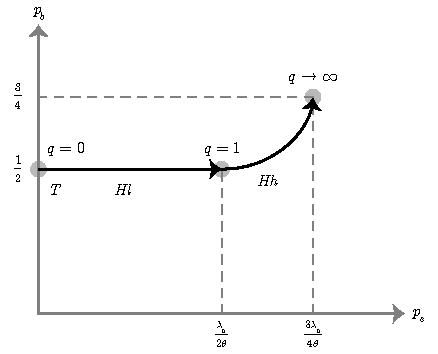
\includegraphics[width = 8.5cm]{old_figure/fig3_price_v2.pdf}
%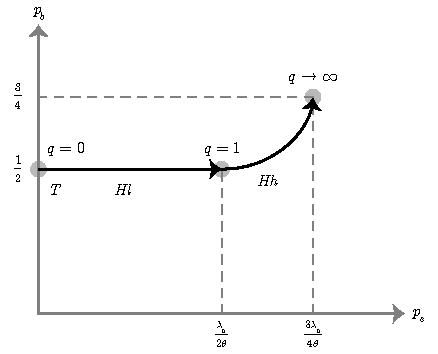
\includegraphics[scale=1.4]{old_figure/fig3_price_v2.pdf}
%\includegraphics[width=11cm]{fig3_price_v1.pdf} 
\textbf{\caption{Pricing Schemes and First-best Prices\label{fig:price}}}
\end{figure}

From this lemma, we derive how the optimal service fees of the profit-maximizing platform change according to each pricing scheme, reflecting different levels of free bandwidth allowance. Figure \ref{fig:price} illustrates how the optimal fees in the first-best prices ($p_s^o, p_b^o$) change as the coefficient of the free bandwidth $q$ increases. First, in the two-part tariff, the platform achieves the highest profit by not imposing the storage fee (i.e., $p_s=0$) and charging the smallest bandwidth fee without any free bandwidth. Since all bandwidth usage is charged, the platform benefits by attracting renters without an initial storage fee.

Second, as the free bandwidth amount increases for $0 \le q \le 1$, the platform adjusts by raising the storage service fee while keeping the same bandwidth fee. This occurs when the platform offers the free-download volume below the lowest bandwidth usage level of all renters $\lambda_0$, so the platform compensates for revenue lost on free bandwidth by increasing the lump-sum storage fee. As a result, all renters pay the same total service cost in this pricing scheme, as is the case of the two-part tariff. Lastly, when free bandwidth surpasses the minimum usage level $\lambda_0$ (i.e., $q >1$), some renters receive complete bandwidth access for free. In response, the platform raises both $p_s$ and $p_b$ to cover this gap. Note that when $q \rightarrow \infty$, hybrid pricing approaches subscription-based pricing, as all renters enjoy free bandwidth.

\subsubsection{Market-clearing Prices}

Now, we consider the situation where renters are rationed by the supply level due to the insufficient number of potential providers in the market compared to the storage demand from renters (i.e., \textit{the market-clearing prices}). We investigate how this supply-side restriction affects the platform's profit and system surplus for the three pricing schemes that we study in this paper.

To do so, we first investigate the required number of providers for the first-best prices. Lemma \ref{lem:threshold} summarizes this result. 

\begin{Lemma}\label{lem:threshold}
The platform's optimal service fees belong to the market-clearing prices when the number of potential providers $n_p$ is lower than the threshold $\psi$, which is calculated as:
\begin{equation*}
\begin{aligned}
    &\psi = \begin{cases}
    \frac{\xi \theta }{\alpha} n_r  &\text{ for the two-part tariff and hybrid pricing with } q\le 1,\\
    \frac{5q^3 -3 q^2 + 3q - 2}{3q^3 + 3q^2 - 3q} \frac{\xi \theta }{\alpha} n_r   &\text{ for hybrid pricing with } q \ge 1,\\
    \frac{5}{3}\frac{\xi \theta }{\alpha} n_r &\text{ for subscription-based pricing,}
    \end{cases}
    \end{aligned}
\end{equation*}
and the optimal service fees of the platform decrease in $n_p$ when $n_p \le \psi$. 
\end{Lemma}

\begin{figure}[ht!]
\centering
%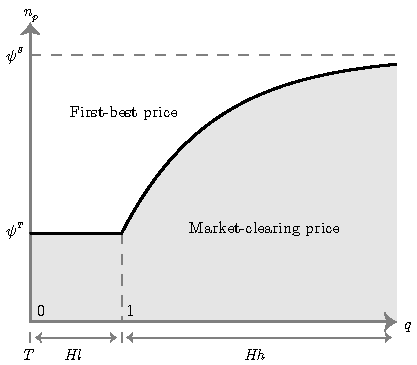
\includegraphics[scale=1.4]{old_figure/fig4_psi_v2.pdf} 
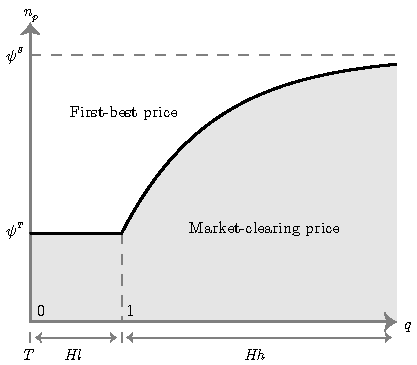
\includegraphics[width=8.5cm]{old_figure/fig4_psi_v2.pdf} 
\textbf{\caption{Free Bandwidth Allowance and First-best Price Thresholds\label{fig:first_best}}}
\end{figure}

For simplicity, we denote the thresholds of the two-part tariff and subscription-based pricing by $\psi^T$ and $\psi^S$, respectively. Figure \ref{fig:first_best} illustrates how the first-best price threshold $n_p$ changes with respect to the coefficient of free bandwidth allowance $q$ in hybrid pricing as shown in Lemma \ref{lem:threshold}. Specifically, when there are ample potential providers in the market compared to the threshold, the platform can achieve the highest profit using the first-best prices. Otherwise, such prices do not sufficiently incentivize providers to satisfy the storage demand from renters. As presented in Figure \ref{fig:first_best}, the threshold increases in $q$, suggesting that a high free bandwidth allowance discourages providers from participating in the platform due to a high operating cost involved with it. We also find that the threshold increases in $\xi \theta$, and it decreases in $\alpha$. Note that $\xi \theta$ is proportional to the total operating cost of providers, while $\alpha$ indicates the providers' revenue share. Therefore, these results indicate that the first-best prices become less feasible as providers' profitability decreases.

When the size of potential providers is insufficient to meet the storage demand from renters, the platform should set the market-clearing prices to incentivize providers. Specifically, for a given pricing scheme, the platform is better off by increasing both $p_s$ and $p_b$ until the number of participating providers equals the number of renters willing to adopt the platform. Alternatively, the platform may incentivize providers by lowering $q$ to fulfill the storage demand from renters (Lemma \ref{lem:threshold}). In that case, since a lower free bandwidth allowance can reduce renters' utility---particularly those with a high usage level, this approach increases service costs imposed on renters.

\subsection{Optimal Redundancy Algorithm}

Recall that the P2P storage platform uses the redundancy rate denoted by $\theta$ and the uptime level $t$ to avoid security problems and ensure a high capacity availability. In this subsection, we consider the platform's endogenous decision on the redundancy algorithm by considering its potential consequences. The redundancy algorithm may affect the behavior of renters and providers in the following ways. First, a higher redundancy rate $\theta$ indicates that each renter contracts with a larger number of providers for the same volume of files. This incurs a higher storage cost to renters and a higher storage revenue to providers, which prohibits renters from adopting the platform. In contrast, an increase in the storage revenue encourages providers to join the platform. Second, the bandwidth volume transmitted through each provider decreases with $\theta$. As $\theta$ increases, more providers share the given bandwidth demand. Therefore, the bandwidth revenue and the operating cost for each provider decrease. Third, a higher $\theta$ leads to a lower uptime $t$ to meet the intended availability level, lowering each provider's operating cost. Here, we derive how the platform should determine the redundancy algorithm in Theorem \ref{thm:redundancy}.

\begin{Theorem}\label{thm:redundancy}
For all pricing schemes, the profit-maximizing redundancy algorithm minimizes the total providers' operating costs in the platform; that is, $\arg\max_{\theta, t} \Pi(p_s^o, p_b^o) = \arg\min_{\theta, t} \xi \theta$.
\end{Theorem}

Recall that we assume that firms only consider $(\theta, t)$ combinations that satisfy the target failure probability, as discussed in Section \ref{subsec:setups}, implying that $\theta > 1$ and $t > 0$. The theorem shows that the platform always decides to set the algorithm to minimize the total operating costs of providers, which is proportional to $\xi \theta$---where $\xi$ is an increasing function of uptime $t$. A lowered operating cost implies that the P2P storage network is more efficient and attractive to potential providers, which leads to a larger number of participating providers. Namely, a lower $\xi \theta$ enables the platform to serve the same number of renters with fewer potential providers and achieve the first-best prices, in line with Lemma \ref{lem:threshold}.

Furthermore, we show that the optimal ($\theta$, $t$) is identical across the pricing schemes. This result is intuitive considering that lowering operating costs helps every stakeholder, and importantly, $\xi \theta$ is not a function of service fees, storage capacity, or usage levels. Based on these findings, we can directly use Lemmas \ref{lem:pricing} and \ref{lem:threshold} to compare these pricing schemes.
%
%
\section{Pricing Schemes, Profit, and System Surplus}\label{sec:analysis2}

Since the P2P storage service uses a two-sided platform with renters and providers, it often matters whether this service improves each stakeholder's surplus. As such, two-sided platforms encounter public controversies regarding whether or not they fairly reward providers \citep{gartenberg2021google, scheiber2015growth}. Moreover, consumers and politicians are concerned about the possibility that customers are unfairly treated by large platforms \citep{kosoff2015newyorkcity}. Considering that such negative sentiments might incur substantive damages to the platform \citep{cachon2017role}, it is important to understand the potential tension between the platform's profit maximization and the other stakeholders' surplus. In this regard, we analyze the impact of pricing schemes on the overall system surplus as well as the platform's profit based on the results in the previous section.

\subsection{Under First-best Prices}

As described in Section \ref{sec:analysis1}, under the given service fees ($p_s, p_b$) and the total storage (paid bandwidth) volume $\upsilon_s$ ($\upsilon_{bp}$), the platform's profit $\Pi$ is:
\begin{equation*}
\Pi(p_s, p_b) = (1-\alpha) (\theta \upsilon_s p_s + \upsilon_{bp} p_b).
\end{equation*}

\noindent While providers obtain the same revenue for the storage service from renters, their operating costs differ across $\rho_j$. Thus, provider $j$ would join the platform when the costs are lower than a certain threshold; that is, $\rho_j \le \rho_m$. Also, the total providers' storage volume used by the service is $V_s = \theta \upsilon_s$. Then, the provider surplus is calculated as:
\begin{equation*}
PS = \frac{\theta \upsilon_s}{\rho_m} \int_{0}^{\rho_m} \left[ \alpha \left(p_s + \frac{\upsilon_{bp}}{\theta \upsilon_s} p_b\right) - \rho \frac{\xi \upsilon_{b}}{\theta \upsilon_s}\right] d\rho.
\end{equation*}

\noindent For renter $i$, the value from service usage is $\lambda_i u_i$ and the service cost $c_i$ depends on the pricing scheme and the service fee ($p_s, p_b$). Her surplus is then calculated as $\lambda_i u_i - c_i$. As $\lambda_i$ and $u_i$ have renter-specific value whose probability distribution functions are $f(\lambda)$ and $1$ (i.e., $u_i \sim U[0, 1]$), respectively, we calculate the total surplus of renter as:
\begin{equation*}
RS = \int_{\lambda} \int_{u(\lambda)} \{\lambda u - c(\lambda, u) \}f(\lambda) du d\lambda.  
\end{equation*}

\noindent Then, we calculate the total surplus $TS$ as the sum of the platform's profit $\Pi$, provider surplus $PS$, and renter surplus $RS$ (i.e., $TS = \Pi + PS + RS$). Using the optimal service fees in each pricing scheme under the first-best prices in Lemma \ref{lem:pricing}, we obtain the platform's profit ($\Pi$) and the total surplus ($TS$) for each pricing scheme. Theorem \ref{thm:surplus_first} below shows the order of the platform's profit and the total system surplus under the first-best prices:

\begin{Theorem}\label{thm:surplus_first} 
Under the first-best prices, the orders of the platform's profit and the total surplus in the three pricing schemes are determined as follows:
\begin{table}[h] \centering
\label{tbl:thm1}
    \begin{tabular}{l  l}
        Platform's profit & $\Pi^S  \le \Pi^{Hh} \le \Pi^{Hl} = \Pi^T $\\
        %Providers' surplus & $PS^S  \le PS^{Hh} \le PS^{Hl} = PS^T $\\
        %Renters' surplus & $RS^T = RS^{Hl} \le RS^{Hh} \le RS^S$\\
        Total surplus & $TS^T = TS^{Hl} \le TS^{Hh} \le TS^S$,
    \end{tabular}
\end{table}

\noindent where superscripts $T$, $Hl$, $Hh$, and $S$ indicate the two-part tariff, hybrid pricing with low $q (\le 1)$, hybrid pricing with high $q (\ge 1)$, and subscription-based pricing, respectively.
\end{Theorem}

The two-part tariff and hybrid pricing with low $q$ yield the same outcomes (i.e., $\Pi^{T} = \Pi^{Hl}$ and $TS^T = TS^{Hl}$). As shown in Lemma \ref{lem
}, when $q < 1$, the free bandwidth allowance is less than any renter's usage level (i.e., $q\lambda_0 < \lambda_0$). Thus, under hybrid pricing with low $q$, the platform can increase $p_s$ enough to recover the lost bandwidth revenue without deterring renters, achieving the same revenue as under the two-part tariff, even with a small free bandwidth allowance.

However, when $q$ exceeds 1, platform profit decreases (i.e., $\Pi^{Hh} \le \Pi^{Hl}$), and total surplus increases (i.e., $TS^{Hh} \ge TS^{Hl}$). With a free bandwidth allowance above $\lambda_0$, some renters can use all their bandwidth without paying extra. To cover this loss, the platform may raise the storage fee, though it does not fully offset the revenue lost from free downloads. In practice, platforms often offer substantial rather than minimal free allowances to attract customers, suggesting that P2P platforms may have limited incentive to use free bandwidth to boost short-term profits. Subscription-based pricing, which provides unlimited free bandwidth, can be viewed as a special case of hybrid pricing. As $q$ approaches infinity, platform profit is minimized, while system surplus is maximized.

Interestingly, all pricing schemes attract the same number of renters under first-best pricing. Thus, differences in total surplus stem from variations in renters' usage levels, not the total number of renters. Specifically, as $q$ increases, higher-usage renters (with higher $\lambda$) are more likely to adopt the platform. This shift means that the added benefit to renters from increasing $q$ outweighs the platform's profit loss, ultimately boosting system surplus.

\subsection{Under Market-clearing Prices}

The consequences of pricing schemes under the market-clearing prices are less straightforward than the first-best prices because service fees can indirectly interact with renter decisions through altering the supply level. We account for this interaction and obtain the following results.

\begin{Theorem}\label{thm:surplus_market}
When the first-best price is not feasible for some pricing schemes, there exist $\underline{\psi}$ as the size of potential providers that satisfy $0 \le \underline{\psi} \le \psi^T < \psi^S$. Then, the platform's profit and total surplus in the three pricing schemes have the following orders.
\begin{enumerate}[label=(\roman*)]
    \item When $n_p$ is moderate such that $\psi^T \le n_p \le \psi^S$, hybrid pricing with $q \ge 1$ can dominate the subscription-based pricing, i.e., $\Pi^{Hh} \ge \Pi^S$ and $TS^{Hh} \ge TS^S$.
    \item When $n_p$ is small such that $\underline{\psi} \le n_p \le \psi^T $, the two-part tariff and hybrid pricing with $q \le 1$ yield higher total surplus than the subscription-based pricing; that is, $TS^T = TS^{Hl} \ge TS^S$. Also, these pricing schemes always ensure higher profits than the subscription-based pricing; that is, $\Pi^T = \Pi^{Hl} \ge \Pi^S$.
\end{enumerate} 
\end{Theorem}

Theorem \ref{thm:surplus_market} suggests that the effectiveness of pricing schemes is highly contingent upon the number of potential providers $n_p$ in the market. When $n_p$ is large such that $n_p \ge \psi^S $, the platform can set the first-best prices. Hence, all results in Theorem \ref{thm:surplus_first} hold, and subscription-based pricing---which creates the renter surplus most---always yields the highest total surplus. However, as $n_p$ decreases, the first-best prices become insufficient to incentivize providers. Hence, the platform should give a higher reward to each provider to maintain the same level of capacity. This result indicates that the size of potential providers needs to be carefully considered in the platform's pricing decisions. 

We further investigate how the optimal service fees in the pricing schemes interplay with $n_p$ and find the following results. First, as $n_p$ is moderate such that $\psi^T \le n_p \le \psi^S$, there exists some hybrid pricing with $q \ge 1$ that outweighs subscription-based pricing in terms of the total surplus as well as the platform's profit. As suggested by Lemma \ref{lem:threshold}, the first-best prices are not applicable for subscription-based pricing when $n_p$ is moderate. Hence, the profit-seeking platform needs to adopt the market-clearing prices to incentivize providers and avoid rationing renters who are willing to pay for the service. Thus, subscription-based pricing experiences a significant decline in the platform's profit, the provider surplus, and the renter surplus. Alternatively, the platform may achieve the first-best prices by reducing the free bandwidth allowance. By balancing the incentive for providers and the renters' utility from the free bandwidth allowance, the platform can achieve a higher total surplus when the number of potential providers is comparable to the number of potential renters.

Second, we show that the two-part tariff, which is equivalent to hybrid pricing with $q \le 1$, can yield the higher surplus than subscription-based pricing when $n_p$ is small such that $\underline{\psi} \le n_p \le \psi^T $. In this case, the platform should attract a large proportion of potential providers to meet the same storage demand from renters. Then, the free bandwidth allowance affects the platform's ability to fulfill the storage demand more adversely. The platform needs to set strikingly high subscription fees to compensate for this adverse effect, and consequently, the renter surplus---the main advantage of subscription-based pricing---substantially decreases. In contrast, the two-part tariff can maintain the required capacity for market-clearing with relatively cheap service fees because it rewards providers for all bandwidth provision. As a consequence, the two-part tariff can achieve a higher system surplus than subscription-based pricing, implying that rewarding providers could be more beneficial to the entire system than focusing on the renter surplus.
%
%
\section{Model Extension: Endogeneous Commission Rates}\label{sec:analysis3}

Thus far, we have assumed an exogenously given commission rate when investigating the platform's optimal service fees. Although it is difficult for two-sided platforms to alter commissions because they often encounter public controversies regarding whether or not they fairly reward providers \citep{gartenberg2021google, scheiber2015growth}, it is still informative to understand how the implications of pricing schemes change when the platform is free to adjust its commission rate. Therefore, in this subsection, we consider an endogenously determined commission rate of the platform. Now, the platform can choose a commission rate to better maximize its profit. Also, it is possible that such a benefit may be amplified under a non-flexible pricing scheme (e.g., subscription-based pricing). To verify the possibility that the endogenous selection of commission rates affects our findings, we re-analyze our model by considering $\alpha$ as a decision variable as well as $p_s$ and $p_b$. Theorem \ref{thm:alpha} summarizes the results according to the exogenous size of potential providers $n_p$. 

\begin{Theorem}\label{thm:alpha}
When the profit-seeking platform endogenously determines the commission rate, there exists $\bar{\psi}_{\alpha}$ as the size of potential providers that satisfies $0 \le \psi_{\alpha}^T \le \bar{\psi}_{\alpha} \le \psi_{\alpha}^S$, where $\psi_{\alpha}^T \equiv \frac{1}{2}\xi \theta n_r$ and $\psi_{\alpha}^S \equiv 3 \xi \theta n_r$. Then, the platform's profit and the total surplus in the three pricing schemes are in the following order.
\begin{enumerate}[label=(\roman*)]
    \item When $n_p$ is large such that $n_p \ge \bar{\psi}_{\alpha}$, the two-part tariff generates the highest platform's profit, while subscription-based pricing yields the highest total surplus (Theorem \ref{thm:surplus_first}).
    \item When $n_p$ is moderate such that  
    $\psi_{\alpha}^T \le n_p \le \bar{\psi}_{\alpha}$, hybrid pricing with some $q \ge 1$ dominates subscription-based pricing. That is, $\Pi^{Hh} \ge \Pi^S$ and $TS^{Hh} \ge TS^S$ (Theorem \ref{thm:surplus_market} (\textit{i})),
    \item When $n_p$ is small such that $0 \le n_p \le \psi_{\alpha}^T$, the two-part tariff and hybrid pricing with $q \le 1$ yield higher total surplus than subscription-based pricing; that is, $TS^T = TS^{Hl} \ge TS^S$. Also, these pricing schemes always ensure higher profits than subscription-based pricing; that is, $\Pi^T = \Pi^{Hl} \ge \Pi^S$ (Theorem \ref{thm:surplus_market} (\textit{ii})).
\end{enumerate}
\end{Theorem}

It shows that the main insights of Theorems \ref{thm:surplus_first} and \ref{thm:surplus_market} continue to hold, although the thresholds for the first-best prices change. This suggests that it is still crucial for the platform to incentivize providers, even when it is free to alter its commission rate to increase its own profit.

While results from endogenous commission rates align with our main findings, they should be interpreted cautiously. First, two-sided platforms must balance profitability with public sentiment, as they often face scrutiny over fair provider compensation \citep{gartenberg2021google, scheiber2015growth}. Second, competitive pressures and regulatory constraints may prevent platforms from setting high commission rates. Even in low-competition environments, insufficient provider rewards could invite new entrants to capture market share. Lastly, high commission rates may be unrealistic; for instance, Sia charges around 3.9\%, and Google Play and Apple's App Store charge 30\%, a rate that has already faced significant backlash \citep{gartenberg2021google}. Thus, commission rates of 67\% or more, as suggested in some scenarios, may not be feasible.\footnote{See Online Appendix \ref{app:proof} for proof details.} These considerations support treating commission rates as exogenous in our model.

\section{Conclusions}

In this study, we developed a game-theoretic model to examine how the P2P storage platform's pricing schemes impact the platform's profit and the total system surplus. We considered three pricing schemes, one of which is widely employed by P2P storage platforms (the two-part tariff), while the others are widely adopted by conventional public cloud services (subscription-based and hybrid pricing). Also, we incorporated endogenous decisions on redundancy algorithms into deciding profit-maximizing service fees under a given pricing scheme.

We found that when ``first-best" prices—those that maximize profit with ample providers—are possible, the two-part tariff maximizes platform profit, while subscription-based pricing achieves the highest total surplus. However, when providers are scarce, the platform cannot use first-best prices and must set market-clearing prices where supply meets demand. In this scenario, two-part tariff and hybrid pricing can outperform subscription-based pricing in terms of both profit and total surplus. To validate these results, we also examined endogenous commission rates and tested our assumptions, confirming that our main insights hold robustly.

Our findings are attributable to the decentralized nature of two-sided platforms. Considering that a two-part tariff can decide both a rump-sum fee and a per-use fee, unlike pay-per-use only in some papers---e.g., \citet{randhawa2008usage}, \citet{cachon2011pricing}, it is intuitive that a firm can convert renter surplus into its profit under two-part tariff than subscription-based pricing. Also, we obtain a higher total surplus from subscription-based pricing under an abundant storage supply, where pricing decisions have a limited impact on the supply level, as expected by the extant literature. In this sense, our finding of when and why the platform's seemingly `greedy' choice may benefit both sides of platform participants is not contradictory to the literature but offers unique insights into P2P markets.

Our findings offer key insights for P2P storage platforms reliant on independent providers and focused on maximizing stakeholder surplus. By comparing the current pricing schemes with alternatives rarely used in P2P storage, we demonstrate that provider scarcity is crucial in determining pricing effectiveness. Specifically, when ample providers are available, a subscription-based model can increase the total system surplus compared to the two-part tariff. However, with limited providers, subscription-based pricing may yield a lower surplus than the two-part tariff or hybrid pricing, which are more profitable for the platform. Additionally, we find that the effectiveness of the pricing scheme is closely tied to the redundancy algorithm; as the algorithm requires higher uptime and redundancy, increasing provider costs, the two-part tariff and hybrid pricing become more advantageous.

These insights provide actionable strategies for platforms, especially given the P2P storage market's early stage. Platforms aiming to grow their user base by increasing total surplus might consider alternative pricing models with higher surplus potential than the two-part tariff. However, if attracting providers proves challenging, possibly due to technical barriers, platforms may need to enhance compensation for bandwidth provision by limiting free bandwidth. It is worth noting that Storj introduced a new pricing scheme wherein renters receive a finite amount of free usage volume. Our results suggest that this change can hardly be supported from a profit-seeking perspective in the short term.

Our research offers managerial insights applicable to other sharing platforms. We find that compensating providers more effectively can increase total surplus, especially when providers are scarcer than consumers. While different pricing schemes are common across platforms, this core principle is transferable. For instance, when few providers bear high operating costs, raising service prices can alleviate this burden. Accordingly, sharing platforms might adopt region-specific pricing strategies. For example, in peer-to-peer delivery platforms, regions with fewer deliverers might improve overall stakeholder surplus and profits by charging sellers or consumers more, while lowering service prices in regions with ample deliverers can increase system surplus.

We conclude by specifying some caveats and potential avenues for future research. First, we have analyzed only a monopoly market. The P2P storage market is highly immature and still rapidly growing, and several new entrants are threatening incumbent players. We expect that future research can significantly benefit from investigating the influence of competitors in this nascent market. 

Second, our model relies on a homogeneous storage volume in order to focus on the interactions between renters and providers. Future studies can make substantial progress by incorporating the heterogeneity of storage volume from the supply and demand sides into their main models. Moreover, our model does not consider the possibility that renters may change their usage levels depending on pricing schemes, which can provide a valuable direction for future research.

Lastly, our results are restricted to three pricing schemes, but many other pricing schemes can be considered. For instance, some public cloud services lower the unit price as the usage level increases in practice. Moreover, cloud platforms may consider offering multiple pricing schemes to differentiate various customer segments more effectively. Analyzing how unexplored pricing schemes affect the platform's profit and system surplus can provide valuable insights.
%
%

%\setlength{\itemsep}{-1pt}%
\setlength{\baselineskip}{15pt}
	\bibliographystyle{informs2014}
%	\bibliographystyle{apacite}
%	\bibliographystyle{pomsref}
	\bibliography{bib}
%
%

\newpage	
\setlength{\baselineskip}{17pt}
\noindent \textbf{\LARGE Online Appendices}
\appendix
\section{Algorithmic Backgrounds}\label{app:algorithm}

{\small % Change font size
\setstretch{1} % Set line spacing to 1

P2P storage platforms typically use erasure coding in their redundancy algorithms to ensure high file availability. In a $k$-of-$m$ erasure coding scheme, a file is divided into $k$ shards, which are then re-coded into $m$ encrypted fragments ($m > k$) \citep{weatherspoon2002erasure, wilkinson2016storj}. Each fragment is assigned to one of $m$ independent providers contracted by the renter. Since any $k$ fragments can reconstruct the file, the platform only requires $k$ providers to be online simultaneously for retrieval. This method achieves high reliability with a low redundancy rate $\theta(=\frac{m}{k})$ \citep{weatherspoon2002erasure}. Given redundancy parameters $k$, $m$, and required uptime $t$, the failure probability can be estimated as follows:

\begin{equation*}
\begin{aligned}
F(t; m, k) = \sum_{j=0}^{k-1} {m \choose j}t^j (1-t)^{m-j}.
\end{aligned}
\end{equation*}

From the equation above, we obtain the following relationships between the failure probability, the redundancy parameters and the required uptime:

\begin{Lemma}\label{lem:uptime}
The failure probability $F(t; m, k)$ is i) decreasing in $t$ for fixed $m$ and $k$, and ii) decreasing in $m$ for fixed $t$ and $k$.
\end{Lemma}

Lemma \ref{lem:uptime} informs about how each parameter impacts failure probability. First, higher required provider uptime reduces failure probability, showing that reliability can be improved by imposing more responsibility on providers while keeping the same redundancy rate. Second, assigning file fragments to more providers also decreases failure probability, indicating that availability can be enhanced by increasing provider numbers instead of boosting individual provider responsibility.

Table \ref{tbl:redundancy_1} shows calculated failure probabilities at $\theta = 3$. Even with constant $\theta$ and uptime $t$, the platform can increase system reliability. For instance, with $\theta=3$ and $t=0.75$, the failure probability is 1.15e-04 when $(k, m) = (5, 15)$. By doubling fragments to $(k, m) = (10, 30)$, the platform reduces failure probability by about 400 times (from 1.15e-04 to 2.82e-07) without changing $\theta$ or $t$. Additionally, a small uptime increase can significantly cut failure probability: under $k=10$ and $m=30$, raising $t$ by 15\%p (from 0.75 to 0.90) reduces failure probability by 48.6 million times (from 2.82e-07 to 5.80e-15).

\begin{table}[h]
\textbf{\caption{An Example of Redundancy Algorithm and Failure Probability ($\theta=3$)\label{tbl:redundancy_1}}}
\begin{center}
\begin{tabular}{cccc|cccc}
 $m$ & $k$ & $t$ & $F(t; m, k)$ & $m$ & $k$ & $t$ & $F(t; m, k)$ \\\hline
15 & 5 & 0.5 & 5.92e-02 & 30 & 10 & 0.5 & 2.14e-02 \\
15 & 5 & 0.75 & 1.15e-04 & 30 & 10 & 0.75 & 2.82e-07 \\
15 & 5 & 0.9 & 9.30e-09 & 30 & 10 & 0.9 & 5.80e-15 \\
15 & 5 & 0.99 & 1.32e-19 & 30 & 10 & 0.99 & 1.31e-35 \\
\end{tabular}
\end{center}
\end{table}

Besides erasure coding, P2P storage platforms implement additional measures to mitigate file transfer failure. Typically, they require providers to meet minimum standards for available storage, processing power, and bandwidth speed. Also, to mandate the uptime level, Sia mandates 95–98\% uptime to ensure 99.9999\% file accessibility; providers failing to maintain 95\% uptime (over 36 hours downtime per month) forfeit their collateral. Storj enforces a stricter 99.3\% uptime (allowing only 5 hours of downtime per month). Filecoin assesses and penalizes providers based on a proof-of-space requirement using miners' collateral. Under these parameters, Sia and Storj are theoretically expected to achieve very low failure probabilities of 2.52e-29 and 2.11e-91 with $(k, m, t)$ values of $(10, 30, 0.98)$ and $(29, 80, 0.993)$, respectively.\footnote{The relevant information was retrieved from the following sources: 1) Storj's redundancy parameters (https://docs.storj.io/concepts/overview), 2) Storj's required uptime (https://www.storj.io/node-operator-terms-conditions), 3) Sia's redundancy parameters (https://support.sia.tech/renting/is-my-data-secure\#security), 4) Sia's required uptime (https://support.sia.tech/hosting/about-hosting-on-sia).} According to Storj, the Tardigrade platform---Storj's main service---demonstrated 99.96\% availability in practice.\footnote{Further details are available at https://www.storj.io/blog/announcing-pioneer-2-and-tardigrade-io-pricing.}

If we assume that the target failure probability $\bar{p}$ is close to zero, i.e., $\bar{p} \approx 0$, the platform's redundancy parameters and the required uptime satisfy the following equation:
\begin{equation*}
\begin{aligned}
F(t; m, k) = \sum_{j=0}^{k-1} {m \choose j}t^j (1-t)^{m-j} \le \bar{p}.
\end{aligned}
\end{equation*}
As shown in Lemma \ref{lem:uptime}, the platform achieves its target failure probability by requiring a high uptime $t$ or adopting a high redundancy rate $\theta$. Table \ref{tbl:redundancy_2} presents the calculated pair of the redundancy rate and the required uptime for $k=10$ and the target probability $\bar{p} = 10e-10$. Figure \ref{fig:redundancy} visualizes this relationship. When a redundancy rate is low, increasing $\theta$ does not significantly decrease the required uptime. For instance, when $\theta$ increases from 1 to 1.5, the required $t$ decreases by only 0.005. In contrast, when we compare $\theta = 3$ and $\theta = 3.5$, the required uptime decreased by (from 0.836 to 0.776).

\begin{table}[h]
\textbf{\caption{An Example of Redundancy Rate and Uptime ($k=10$, $\bar{p} = 10^{-10}$)\label{tbl:redundancy_2}}}
\begin{center}
\begin{tabular}{ccc|ccc|ccc|ccc}
 $\theta$ &$t$&$\theta$ & $t$&$\theta$&$t$ & $t$&$\theta$&$t$ & $t$&$\theta$&$t$ \\ \hline
$\le$1.2 & 1 & 2.0 & 1.6 & 0.990 & 2.4 & 0.957 & 2.8 & 0.861 & 0.911 & 3.2 & 0.812\\
1.3 & 0.999 & 2.1 & 1.7 & 0.984 & 2.5 & 0.947 & 2.9 & 0.849 & 0.899 & 3.3 & 0.800 \\
1.4 & 0.998 & 2.2 & 1.8 & 0.976 & 2.6 & 0.935 & 3.0 & 0.836 & 0.886 & 3.4 & 0.788 \\
1.5 & 0.995 & 2.3 & 1.9 & 0.967 & 2.7 & 0.924 & 3.1 & 0.824 & 0.874 & 3.5 & 0.776 \\
\end{tabular}
\end{center}
\end{table}

\begin{figure}[ht!]
\centering
\includegraphics[width=9cm]{figure_3rd_final/uptime_fig.jpg} 
\textbf{\caption{Redundancy Rate and Required Uptime ($k=10$, $\bar{p} = 10^{-10}$)\label{fig:redundancy}}}
\end{figure}

}

%\newpage
\section{Proof}\label{app:proof}

{\small % Change font size
\setstretch{1} % Set line spacing to 1

\paragraph{Proof of Lemma \ref{lem:pvd_chr}}
\begin{proof}
As provider \textit{j}'s cost increases in $\rho_j$, if $\pi|_{\rho_j = 1} \ge 0$, all providers are profitable (i.e., $\rho_m = 1$). If $\pi|_{\rho_j= 1} <0$, there exists $\rho_m < 1$ that satisfies $\pi|_{\rho_j = \rho_m} = 0$. Also, if $\omega_s \le \theta \upsilon_s $, all providers' utilization becomes $1$. When $\theta \upsilon_s < \omega_s $, all providers' utilization is strictly lower than $1$. We thus consider these cases:
\begin{table}[h]
\begin{center}
\begin{tabular}{c|cc}
&$\pi|_{\rho_j = 1} \ge 0$ & $\pi|_{\rho_j = 1} < 0$\\\hline 
$\omega_s \le \theta \upsilon_s$ & $\rho_m = 1$, $\hat{\omega}_s=1 $ & $\rho_m < 1$, $\hat{\omega}_s=1 $\\
$\theta \upsilon_s < \omega_s$& $\rho_m = 1$, $\hat{\omega}_s<1 $ & $\rho_m < 1$, $\hat{\omega}_s<1 $\\
\end{tabular}
\end{center}
\end{table}

\noindent \textbf{A. Analysis of Cases and Sub-conditions}\\

\noindent \textbf{\textit{Case A1:}} $\pi|_{\rho_j =1} \ge 0$ and $\omega_s \le \theta \upsilon_s$. 

\noindent This condition leads to $\rho_m = 1$ and $\hat{\omega}_s = 1$. For each of the two sub-conditions, we obtain the followings:

\textit{\underline{Sub-condition A1-i:}} $\pi|_{\rho_j = 1} \ge 0$:
\begin{equation*}
\begin{aligned}
&\pi|_{\rho_j = 1} \ge 0 \Leftrightarrow \alpha p_s + \alpha p_b \frac{\upsilon_{bp}}{\theta \upsilon_s} - \frac{\xi \upsilon_b}{\theta \upsilon_s} \ge 0 \Leftrightarrow \frac{\xi \upsilon_b}{\theta \upsilon_s} \le \alpha p_s + \alpha p_b \frac{\upsilon_{bp}}{\theta \upsilon_s} \Leftrightarrow g_1 \le \tilde{\pi}, 
\end{aligned}
\end{equation*}

\textit{\underline{Sub-condition A1-ii:}} $\omega_s \le \theta \upsilon_s$:
\begin{equation*}
\begin{aligned}
&\omega_s \le \theta \upsilon_s \Leftrightarrow n_p \le \theta \upsilon_s.
\end{aligned}
\end{equation*}

As a result, we obtain $(\rho_m, \hat{\omega}_s) = (1, 1)$.\\

\noindent \textbf{\textit{Case A2:}} $\pi|_{\rho_j =1} <0$ and $\omega_s \le \theta \upsilon_s$.\\
\noindent In this condition, $\rho_m <1$ and $\hat{\omega}_s = 1$. Then, the sub-conditions lead to the following results:

\textit{\underline{Sub-condition A2-i:}} $\pi|_{\rho_j = \rho_m} = 0$ where $\rho_m < 1$: 
\begin{equation*}
\begin{aligned}
&\pi|_{\rho_j = \rho_m} = 0 \Leftrightarrow \alpha p_s + \alpha p_b \frac{\upsilon_{bp}}{\theta \upsilon_s} - \rho_m \frac{\xi \upsilon_b}{\theta \upsilon_s} = 0 \Leftrightarrow \rho_m = \frac{\alpha p_s + \alpha p_b \frac{\upsilon_{bp}}{\theta \upsilon_s}}{\frac{\xi \upsilon_b}{\theta \upsilon_s}} \Rightarrow \rho_m < 1 \Leftrightarrow \frac{\alpha p_s + \alpha p_b \frac{\upsilon_{bp}}{\theta \upsilon_s}}{\frac{\xi \upsilon_b}{\theta \upsilon_s}} < 1 \Leftrightarrow \tilde{\pi}<g_1,
\end{aligned}
\end{equation*} 

\textit{\underline{Sub-condition A2-ii:}} $\omega_s \le \theta \upsilon_s$:
\begin{equation*}
\begin{aligned}
&\omega_s \le \theta \upsilon_s \Leftrightarrow n_p \rho_m \le \theta \upsilon_s \Leftrightarrow n_p \frac{\alpha p_s + \alpha p_b \frac{\upsilon_{bp}}{\theta \upsilon_s}}{\frac{\xi \upsilon_b}{\theta \upsilon_s}} \le \theta \upsilon_s \Leftrightarrow \alpha p_s + \alpha p_b \frac{\upsilon_{bp}}{\theta \upsilon_s}  \le \frac{\xi \upsilon_b}{n_p} \Leftrightarrow \tilde{\pi} \le g_2. 
\end{aligned}
\end{equation*}

It follows that $(\rho_m, \hat{\omega}_s) = (\frac{\tilde{\pi}}{g_1}, 1)$.\\

\noindent \textbf{\textit{Case A3:}} $\pi|_{\rho_j =1} \ge 0$ and $\theta \upsilon_s < \omega_s $.\\
This condition results in $\rho_m = 1$ and $\hat{\omega}_s = \frac{\theta \upsilon_s}{\omega_s}$. The two sub-conditions lead to the followings:

\textit{\underline{Sub-condition A3-i:}} $\pi|_{\rho_j = 1} \ge 0$:
\begin{equation*}
\begin{aligned}
&0 \le \pi|_{\rho_j = 1} \Leftrightarrow 0 \le \alpha p_s + \alpha p_b \frac{\upsilon_{bp}}{\theta \upsilon_s} - \frac{\xi \upsilon_b}{\theta \upsilon_s} \Leftrightarrow \frac{\xi \upsilon_b}{\theta \upsilon_s} \le \alpha p_s + \alpha p_b \frac{\upsilon_{bp}}{\theta \upsilon_s} \Leftrightarrow g_1 \le \tilde{\pi}, 
\end{aligned}
\end{equation*}

\textit{\underline{Sub-condition A3-ii:}} $ \theta \upsilon_s < \omega_s$:
\begin{equation*}
\begin{aligned}
&\theta \upsilon_s < \omega_s \Leftrightarrow \theta \upsilon_s < n_p.
\end{aligned}
\end{equation*}

Then, $ (\rho_m, \hat{\omega}_s) = (1, \frac{\theta \upsilon_s}{n_p})$.\\

\noindent \textbf{\textit{Case A4:}} $\pi|_{\rho_j =1} <0$ and $\theta \upsilon_s < \omega_s $.\\
This condition leads to $\rho_m <1$ and $\hat{\omega}_s = \frac{\theta \upsilon_s}{\omega_s}$. For the two sub-conditions, we obtain the followings:

\textit{\underline{Sub-condition A4-i:}} $\pi|_{\rho_j = \rho_m} = 0$ where $\rho_m < 1$:
\begin{equation*}
\begin{aligned}
&\pi|_{\rho_j = \rho_m} = 0 \Leftrightarrow \alpha p_s + \alpha p_b \frac{\upsilon_{bp}}{\theta \upsilon_s} - \rho_m \frac{\xi \upsilon_b}{\theta \upsilon_s} = 0 \Leftrightarrow \rho_m = \frac{\alpha p_s + \alpha p_b \frac{\upsilon_{bp}}{\theta \upsilon_s}}{\frac{\xi \upsilon_b}{\theta \upsilon_s}} \Rightarrow \rho_m < 1 \Leftrightarrow \frac{\alpha p_s + \alpha p_b \frac{\upsilon_{bp}}{\theta \upsilon_s}}{\frac{\xi \upsilon_b}{\theta \upsilon_s}} < 1 \Leftrightarrow \tilde{\pi} < g_1,
\end{aligned}
\end{equation*}

\textit{\underline{Sub-condition A4-ii:}} $\theta \upsilon_s < \omega_s$: 
\begin{equation*}
\begin{aligned}
&\theta \upsilon_s < \omega_s \Leftrightarrow \theta \upsilon_s < n_p \rho_m \Leftrightarrow \theta \upsilon_s < n_p \frac{\alpha p_s + \alpha p_b \frac{\upsilon_{bp}}{\theta \upsilon_s}}{\frac{\xi \upsilon_b}{\theta \upsilon_s}} \Leftrightarrow   \frac{\xi \upsilon_b}{n_p}  <   \alpha p_s + \alpha p_b \frac{\upsilon_{bp}}{\theta \upsilon_s} \Leftrightarrow g_2 < \tilde{\pi}.   
\end{aligned}
\end{equation*}

Therefore, we observe that $ (\rho_m, \hat{\omega}_s) = (\frac{\tilde{\pi}}{g_1}, \frac{g_2}{\tilde{\pi}} )$. \\

\noindent \textbf{B. Feasibility Analysis}\\
Since $\theta \upsilon \lessgtr n_p \Leftrightarrow g_2 \lessgtr g_1$ holds, we consider the following cases:\\

\noindent \textbf{\textit{Case B1:}} $\theta \upsilon_s \le n_p$.\\
This case implies $g_2 \le g_1$. Using this property, we analyze the feasible region for each of the cases in part A:

\textbf{\textit{Case A1:}} infeasible,

\textbf{\textit{Case A2:}} when $\tilde{\pi} \le g_2$, $(\rho_m, \hat{\omega}_s) = (\frac{\tilde{\pi}}{g_1}, 1)$,

\textbf{\textit{Case A3:}} when $g_1 \le \tilde{\pi}$, $(\rho_m, \hat{\omega}_s) = (1, \frac{\theta \upsilon_s}{n_p})$,

\textbf{\textit{Case A4:}} when $g_2 < \tilde{\pi} < g_1$, $(\rho_m, \hat{\omega}_s) = (\frac{\tilde{\pi}}{g_1}, \frac{g_2}{\tilde{\pi}})$.

These feasible regions and the continuity of $(\rho_m, \hat{\omega}_s)$ lead to the results for $\theta \upsilon_s \le n_p$ in Lemma \ref{lem:pvd_chr}.\\

\noindent \textbf{\textit{Case B2:}} $\theta \upsilon_s \ge n_p$.
In this case, we see $g_2 \ge g_1$. For each case in the part A, the feasible region is:

\textbf{\textit{Case A1:}} when $g_1 \le \tilde{\pi}$, $(\rho_m, \hat{\omega}_s) = (1, 1)$,

\textbf{\textit{Case A2:}} when $\tilde{\pi} < g_1$, $(\rho_m, \hat{\omega}_s) = (\frac{\tilde{\pi}}{g_1}, 1)$,

\textbf{\textit{Case A3, Case A4:}} infeasible.

These feasible regions and the continuity of $(\rho_m, \hat{\omega}_s)$ lead to the results for $n_p \le \theta \upsilon_s$ in Lemma \ref{lem:pvd_chr}.
\end{proof}


\paragraph{Proof of Lemma \ref{lem:pricing}}
\begin{proof}
We derive the profit-maximizing service fees for each pricing scheme. In doing so, we separate hybrid pricing into two cases based on whether the free bandwidth allowance exceeds the minimum usage level $\lambda_0$.\\  

\noindent \textbf{\textit{Case 1: The two-part tariff.}}\\

\textit{\underline{Sub-case 1-i:}} $0 \le p_s \le \frac{\lambda_0 - \lambda_0 p_b}{\theta}$.

The total storage volume $\upsilon_s$ and the total paid bandwidth volume $\upsilon_{bp}$ are derived as follows:

\begin{equation*}
\begin{aligned}
&\upsilon_s = n_r \int_{\lambda_0}^{\infty}(1-\frac{\theta p_s}{\lambda} - p_b) f(\lambda) d \lambda = n_r(1-\frac{2\theta p_s}{3\lambda_0} - p_b),\\
&\upsilon_{bp} = n_r \int_{\lambda_0}^{\infty}\lambda (1-\frac{\theta p_s}{\lambda} - p_b) f(\lambda) d \lambda  = n_r\left[-\theta p_s + 2\lambda_0 (1-p_b) \right].
\end{aligned}
\end{equation*}

Using the derived $\theta \upsilon_s$ and $\upsilon_{bp}$, we can rewrite the platform's objective function as $\max_{p_s, p_b}\Pi(p_s, p_b) = (1-\alpha) \theta n_r \left( - \frac{2\theta}{3\lambda_0} p_s^2 - 2 p_s p_b - \frac{2\lambda_0}{\theta} p_b^2 + p_s + \frac{2\lambda_0}{\theta} p_b\right)$.

Then, we verify the second-order condition by analyzing the Hessian matrix of that profit function
\begin{equation*}
H=\begin{bmatrix}
-\frac{4(1-\alpha) \theta^2 n_r}{3\lambda_0} & -2(1-\alpha) \theta n_r\\
-2(1-\alpha) \theta n_r & -4 (1-\alpha) \lambda_0 n_r
\end{bmatrix}.
\end{equation*}

We observe that the first-order leading principal minor is negative and the second-order leading principal minor is $det(H) = \frac{4}{3}(1-\alpha)^2 \theta^2 n_r^2 >0$. Thus, $H$ is negative-definite, the second-order condition is satisfied, and this profit function has the global maximum. Consequently, the optimal service fee is $\left(p_s^T, p_b^T\right) = \left(0, \frac{1}{2}\right)$.

\textit{\underline{Sub-case 1-ii:}} $p_s \ge \frac{\lambda_0 - \lambda_0 p_b}{\theta} $.

% In this sub-case, $\upsilon_s$ and $\upsilon_{bp}$ are derived as follows:
% \begin{equation*}
% \begin{aligned}
% &\upsilon_s = n_r \int_{\lambda^S}^{\infty}(1-\frac{\theta p_s}{\lambda} - p_b) f(\lambda) d \lambda = \frac{n_r \lambda_0^2(1-p_b)^3}{3\theta^2 p_s^2},\\
% &\upsilon_{bp} = n_r \int_{\lambda^S}^{\infty}\lambda (1-\frac{\theta p_s}{\lambda} - p_b) f(\lambda) d \lambda  = \frac{n_r(1-p_b)^2 \lambda_0^2}{\theta p_s}.
% \end{aligned}
% \end{equation*}

% Putting $\theta \upsilon_s$ and $\upsilon_{bp}$ into the objective function, the platform's objective is re-written as:

We can derive $\upsilon_s$ and $\upsilon_{bp}$ and rewrite the platform's objective as $\max_{p_s, p_b}\Pi(p_s, p_b) = \frac{n_r(1-\alpha) \lambda_0^2 (1-p_b)^2(1+2p_b)}{3 \theta p_s}$. Since $\Pi(p_s, p_b)$ is decreasing in $p_s$ for all $p_b$, the optimal storage fee satisfies $p_s^T = \frac{\lambda_0 - \lambda_0 p_b}{\theta}$. This is dominated by \textit{Sub-case 1-i} since the optimal storage fee satisfies the boundary condition of the previous sub-case. \\

\noindent \textbf{\textit{Case 2: Subscription-based pricing.}}\\
Similarly, we divide the current case into two sub-cases based on the storage service fee $p_s$ as:

\textit{\underline{Sub-case 2-i:}} $0 \le p_s \le \frac{\lambda_0}{\theta}$.

The total storage volume of renters willing to adopt the platform $\upsilon_s$ is calculated as $\upsilon_s = n_r \int_{\lambda_0}^{\infty} (1-\frac{\theta p_s}{\lambda}) f(\lambda) d\lambda = n_r(1-\frac{2 \theta p_s}{3\lambda_0})$. Then, we rewrite it as $\max_{p_s}\Pi(p_s) = (1-\alpha) \theta n_r \left(- \frac{2\theta}{3 \lambda_0} p_s^2 + p_s\right)$ by putting $\upsilon_s$ into the objective function. 
Since the objective function is concave with respect to $p_s$, the optimal storage fee in this pricing scheme is obtained at $p_s^S = \frac{3\lambda_0}{4\theta}$.\\

\textit{\underline{Sub-case 2-ii:}} $p_s \ge \frac{\lambda_0}{\theta}$.

%The $\upsilon_s$ is calculated as follows:
%\begin{equation*}
%    \upsilon_s = n_r \int_{\lambda^S}^{\infty} (1-\frac{\theta p_s}{\lambda}) f(\lambda) d\lambda = \frac{n_r \lambda_0^2}{3 \theta^2 p_s^2}.
%\end{equation*}

%Putting $\upsilon_s$ into the objective function, we can express the platform's objective as:

We can derive $\upsilon_s$ and rewrite the platform's objective as $\max_{p_s}\Pi(p_s) = \frac{(1-\alpha) n_r \lambda_0^2}{3 \theta p_s}$. Since the objective function is decreasing in $p_s$, the optimal service fee in this sub-case is obtained at $p_s^S = \frac{\lambda_0}{\theta}$. Note that this sub-case is dominated by \textit{Sub-case 2-i} because $p_s^S= \frac{\lambda_0}{\theta}$ is the boundary condition the previous sub-case. Thus, the optimal service fee for subscription-based pricing is obtained as Lemma \ref{lem:pricing}.\\


\noindent \textbf{\textit{Case 3: Hybrid pricing with small free bandwidth allowance ($q \le 1$).}}\\
This pricing is divided into the two sub-cases by the storage service fee $p_s$ show the following results:

\textit{\underline{Sub-case 3-i:}} $0 \le p_s \le \frac{\lambda_0 - (1-q)\lambda_0 p_b}{\theta}$.

$\upsilon_s$ and $\upsilon_{bp}$ are derived as follows:
\begin{equation*}
\begin{aligned}
    &\upsilon_s = \int_{\lambda_0}^{\infty}\{1-\frac{\theta p_s + p_b(\lambda - q \lambda_0)}{ \lambda}\}f(\lambda) d \lambda = n_r\left[1-\frac{2 \theta p_s}{3\lambda_0}-\frac{3-2q}{3} p_b\right],\\
    &\upsilon_{bp} = \int_{\lambda_0}^{\infty}\{1-\frac{\theta p_s + p_b(\lambda - q \lambda_0)}{ \lambda}\}(\lambda - q \lambda_0) f(\lambda) d \lambda = n_r \left[(2-q)\lambda_0 - \frac{1}{3}(3-2q) \theta p_s - \frac{2}{3}(3 - 3q + q^2) \lambda_0 p_b \right].
    \end{aligned}
\end{equation*}

The platform's objective function as $\max_{p_s, p_b}\Pi(p_s, p_b) = (1-\alpha) \theta n_r \{ - \frac{2\theta}{3\lambda_0} p_s^2 - (2-\frac{4q}{3}) p_s p_b - \frac{2(3 - 3q + q^2)\lambda_0}{3\theta} p_b^2 + p_s + \frac{(2-q)\lambda_0}{\theta} p_b\}$ can be obtained by using the derived $\upsilon_s$ and $\upsilon_{bp}$. Then, we verify the second-order condition by analyzing the Hessian matrix of that profit function:
\begin{equation*}
H=\begin{bmatrix}
-\frac{4(1-\alpha) \theta^2 n_r}{3\lambda_0} & -\frac{6-4q}{3}(1-\alpha) \theta n_r\\
-\frac{6-4q}{3}(1-\alpha) \theta n_r & -\frac{2(3-3q+q^2)}{3} (1-\alpha) \lambda_0 n_r
\end{bmatrix}.
\end{equation*}

The first-order leading principal minor is negative and the second-order leading principal minor is $det(H) = \frac{4}{3}(1-\alpha)^2 \theta^2 n_r^2 >0$. It follows that $H$ is negative-definite, and the second-order condition is satisfied. Consequently, this profit function has a global maximum, and we can obtain the optimal price as $\left(p_s^{Hl}, p_b^{Hl}\right) = \left(\frac{q \lambda_0}{2\theta}, \frac{1}{2}\right)$.

\textit{\underline{Sub-case 3-ii:}} $p_s \ge \frac{\lambda_0 - (1-q)\lambda_0 p_b}{\theta}$.

% We can derive $\upsilon_s$ and $\upsilon_{bp}$ as follows:
% \begin{equation*}
% \begin{aligned}
%    &\upsilon_s = \int_{\lambda^{H}}^{\infty}\{1-\frac{\theta p_s + p_b(\lambda - q \lambda_0)}{ \lambda}\}f(\lambda) d \lambda = \frac{n_r \lambda_0^2 (1-p_b)^3}{3(\theta p_s - q \lambda_0 p_b)^2},\\
%    &\upsilon_{bp} = \int_{\lambda_0}^{\infty}\{1-\frac{\theta p_s + p_b(\lambda - q \lambda_0)}{ \lambda}\}(\lambda - q \lambda_0) f(\lambda) d \lambda = \frac{n_r \lambda_0^2(1-p_b)^2(3 \theta p_s - 2 q \lambda_0 p_b - q \lambda_0)}{3(\theta p_s - q \lambda_0 p_b)^2}.
%    \end{aligned}
%\end{equation*}

%The obtained $\upsilon_s$ and $\upsilon_{bp}$ lead to the following objective function:
We can rewrite the objective function as $\max_{p_s, p_b}\Pi(p_s, p_b) = \frac{(1-\alpha) n_r \lambda_0^2(1-p_b)^2(1+2p_b)}{3 \theta p_s - 3 q \lambda_0 p_b}$ by deriving $\upsilon_s$ and $\upsilon_{bp}$. Here, we see $3 \theta p_s - 3 q \lambda_0 p_b \ge 3 \lambda_0 - 3 \lambda_0 p_b \ge 0$, indicating that the denominator is positive. Thus, the objective function is decreasing in $p_s$ for all $p_b$. Also, the optimal storage fee is $p_s^H = \frac{\lambda_0 - (1-q)\lambda_0 p_b}{\theta}$. Since the current sub-case satisfies the boundary condition of \textit{Sub-case 3-i}, the previous sub-case is dominant.\\

\noindent \textbf{\textit{Case 4: Hybrid pricing with large free bandwidth allowance ($q \ge 1$).}}\\
We divide it into three sub-cases based on the storage service fee $p_s$:

\textit{\underline{Sub-case 4-i:}} $0 \le p_s \le \frac{\lambda_0}{\theta}$.

$\upsilon_s$ and $\upsilon_{bp}$ are derived as follows:
\begin{equation*}
\begin{aligned}
&\upsilon_s = \int_{\lambda_0}^{q \lambda_0} \{1-\frac{\theta p_s}{\lambda}\} f(\lambda) d \lambda + \int_{q \lambda_0}^{\infty} \{1-\frac{\theta p_s+p_b(\lambda - q \lambda_0) }{\lambda}\} f(\lambda) d \lambda = n_r(1-\frac{2 \theta p_s}{3 \lambda_0} - \frac{p_b}{3q^2}), \\
&\upsilon_{bp} =  \int_{q \lambda_0}^{\infty}  \{1-\frac{\theta p_s+p_b(\lambda - q \lambda_0) }{\lambda}\} (\lambda - q \lambda_0)f(\lambda) d \lambda = \frac{n_r}{3q^2}(3q\lambda_0 - \theta p_s - 2 q \lambda_0 p_b).
\end{aligned}
\end{equation*}

We obtain the objective function, $\max_{p_s, p_b}\Pi(p_s, p_b) = (1-\alpha) \theta n_r \left( - \frac{2\theta}{3\lambda_0} p_s^2 - \frac{2}{3q^2} p_s p_b - \frac{2\lambda_0}{3 q \theta} p_b^2 + p_s + \frac{\lambda_0}{q \theta} p_b\right)$, by putting $\upsilon_s$ and $\upsilon_{bp}$. Then, we verify the second-order condition by analyzing the following Hessian matrix:
\begin{equation*}
H=\begin{bmatrix}
-\frac{4(1-\alpha) \theta^2 n_r}{3\lambda_0} & -\frac{6-4q}{3}(1-\alpha) \theta n_r\\
-\frac{6-4q}{3}(1-\alpha) \theta n_r & -\frac{2(3-3q+q^2)}{3} (1-\alpha) \lambda_0 n_r
\end{bmatrix}.
\end{equation*}

The first-order leading principal minor is negative and the second-order leading principal minor is $det(H) = \frac{4(4q^3-1)}{9q^4}(1-\alpha)^2 \theta^2 n_r^2 >0$ for $q \ge 1$. Thus, $H$ is negative-definite, and the second-order condition is satisfied. As a result, this profit function has a global maximum. The optimal pricing is $(p_s^{Hh}, p_b^{Hh}) = (\frac{3q(2q^2-1)}{2(4q^3-1)}\frac{\lambda_0}{\theta}, \frac{3q^2(2q-1)}{2(4q^3-1)})$.

\textit{\underline{Sub-case 4-ii:}} $\frac{\lambda_0}{\theta} \le p_s \le \frac{q \lambda_0}{\theta}$.

% The second sub-case has the following $\upsilon_s$ and $\upsilon_{bp}$:
% \begin{equation*}
% \begin{aligned}
% &\upsilon_s = \int_{\lambda^S}^{q \lambda_0} \{1-\frac{\theta p_s}{\lambda}\} f(\lambda) d \lambda + \int_{q \lambda_0}^{\infty} \{1-\frac{\theta p_s+p_b(\lambda - q \lambda_0) }{\lambda}\} f(\lambda) d \lambda = \frac{n_r}{3}\left(\frac{\lambda_0^2}{\theta^2 p_s^2} - \frac{p_b}{q^2} \right), \\
% &\upsilon_{bp} =  \int_{q \lambda_0}^{\infty}  \{1-\frac{\theta p_s+p_b(\lambda - q \lambda_0) }{\lambda}\} (\lambda - q \lambda_0)f(\lambda) d \lambda = \frac{n_r}{3q^2}(3q\lambda_0 - \theta p_s - 2 q \lambda_0 p_b).
% \end{aligned}
% \end{equation*}

% Based on these results, we can rewrite the platform's objective function as
We can derive $\upsilon_s$ and $\upsilon_{bp}$ and rewrite the objective function as $\max_{p_s, p_b} \Pi(p_s, p_b) = - \frac{n_r(1-\alpha)}{3 q^2 \theta p_s}\{2 \theta^2 p_b p_s^2 + q \theta \lambda_0 p_b(2p_b-3) p_s - q^2 \lambda_0^2\}$. Since $\frac{\partial}{\partial p_s}\Pi(p_s, p_b) = - \frac{n_r(1-\alpha)}{3\theta}(\frac{2\theta^2 p_b}{q^2} + \frac{\lambda_0^2}{p_s^2}) \le 0$, this function is decreasing in $p_s$ for all $p_b$. Thus, the optimal storage fee is obtained at $p_s^H = \frac{\lambda_0}{\theta}$. It is dominated by \textit{Sub-case 4-i} since $p_s^H$ satisfies the boundary condition of the previous case.\\

\textit{\underline{Sub-case 4-iii:}} $\frac{q\lambda_0}{\theta} \le p_s $.

% The last sub-case has the following $\upsilon_s$ and $\upsilon_{bp}$:

% \begin{equation*}
% \begin{aligned}
%    &\upsilon_s = \int_{\lambda^{H}}^{\infty}\{1-\frac{\theta p_s + p_b(\lambda - q \lambda_0)}{ \lambda}\}f(\lambda) d \lambda = \frac{n_r \lambda_0^2 (1-p_b)^3}{3(\theta p_s - q \lambda_0 p_b)^2},\\
%    &\upsilon_{bp} = \int_{\lambda_0}^{\infty}\{1-\frac{\theta p_s + p_b(\lambda - q \lambda_0)}{ \lambda}\}(\lambda - q \lambda_0) f(\lambda) d \lambda = \frac{n_r \lambda_0^2(1-p_b)^2(3 \theta p_s - 2 q \lambda_0 p_b - q \lambda_0)}{3(\theta p_s - q \lambda_0 p_b)^2}.
%    \end{aligned}
% \end{equation*}

% Using the derived $\upsilon_s$ and $\upsilon_{bp}$, we can express the platform's objective function as

We can derive $\upsilon_s$ and $\upsilon_{bp}$ and rewrite the platform's objective as $\max_{p_s, p_b} \Pi(p_s, p_b) = \frac{(1-\alpha) n_r \lambda_0^2 (1-p_b)^2 (1+2p_b)}{3 \theta p_s - 3 q \lambda_0 p_b}$. In this region, the denominator is positive or $3 \theta p_s - 3 q \lambda_0 p_b \ge 0$. Thus, the objective function is decreasing in $p_s$ for all $p_b$ and the optimal storage fee is obtained at $\frac{q \lambda_0}{\theta}$. This sub-case is dominated by \textit{Sub-case 4-ii} since the optimal storage fee satisfies the boundary condition of the previous sub-case.
\end{proof}

\paragraph{Proof of Lemma \ref{lem:threshold}}
\begin{proof}
To derive the threshold $\psi$, it suffices to find the $n_p$ which satisfies $\tilde{\pi}(p_s^o, p_b^o; n_p) = g_2(p_s^o, p_b^o; n_p)$. By putting the first-best prices and the corresponding volumes---$\upsilon_s$, $\upsilon_{b}$, and $\upsilon_{bp}$---into $\tilde{\pi}$ and $g_2$, we obtain the threshold $\psi$ in this lemma. To prove that the market-clearing prices are decreasing in $n_p$, we analyze the optimal service fees for each pricing scheme as below:\\

\noindent \textbf{\textit{Case 1: The Two-part Tariff.}}\\
Given that the market-clearing prices satisfies $\tilde{\pi}(p_s, p_b) = g_2(p_s, p_b)$, we obtain the storage fee $p_s$ as the function of $p_b$ by considering two sub-cases as follows:

\textit{\underline{Sub-case 1-i:}} $p_s \le \frac{\lambda_0 - \lambda_0 p_b}{\theta}$.

In this case, we can express $p_s$ as:
\begin{equation*}
\begin{aligned}
    &p_s = \frac{\lambda_0}{4\theta(\alpha n_p + \xi \theta n_r)}\left[ 3\alpha n_p (1-2p_b) + 7 \xi \theta n_r (1-p_b) \right.\\
    &\left. - \sqrt{-(12 \alpha^2 n_p^2 + 12 \alpha \xi n_p \theta n_r + 2 \xi^2 \theta^2 n_r^2 ) p_b^2 +2(6\alpha^2 n_p^2 + 9 \alpha \xi n_p \theta n_r - \xi^2 \theta^2 n_r^2) p_b + (3\alpha n_p - \xi \theta n_r)^2}\right].
    \end{aligned}
\end{equation*}

Using these results, we can rewrite the profit function as:\\
\begin{equation*}
\begin{aligned}
    &\Pi(p_b, p_s^o) = \frac{(1-\alpha) \xi \theta n_r^2 \lambda_0 }{12(\alpha n_p + \xi \theta n_r)^2} \left[ (6\alpha n_p + 7 \xi \theta n_r) p_b^2 - (3\alpha n_p + 11 \xi \theta n_r) p_b - 12 \alpha n_p + 4 \xi \theta n_r\right.\\
    &\left. (4-p_b) \sqrt{-(12 \alpha^2 n_p^2 + 12 \alpha \xi n_p \theta n_r + 2 \xi^2 \theta^2 n_r^2 ) p_b^2 +2(6\alpha^2 n_p^2 + 9 \alpha \xi n_p \theta n_r - \xi^2 \theta^2 n_r^2) p_b + (3\alpha n_p - \xi \theta n_r)^2}\right]. 
    \end{aligned}
\end{equation*}

Then, from the first order condition, we obtain the optimal service fee that is feasible for $n_p$ that satisfies $\frac{\xi \theta n_r}{6 \alpha} \le n_p \le \frac{\xi \theta n_r }{\alpha }$ as below:
\begin{equation*}
    \begin{aligned}
    &p_s^T = \frac{3\lambda_0 \{12 \alpha^2 n_p^2 - 28 \alpha n_p \xi \theta n_r + \xi^2 \theta^2 n_r^2 + (2\alpha n_p + \xi \theta n_r)\sqrt{180 \alpha^2 n_p^2 - 12 \alpha n_p \xi \theta n_r + \xi^2 \theta^2 n_r^2} \}}{8\theta (12 \alpha^2 n_p^2 + 12 \alpha n_p \xi \theta n_r - \xi^2 \theta^2 n_r^2)},\\
    &p_b^T = \frac{12 \alpha^2 n_p^2 + 24 \alpha n_p \xi \theta n_r - 3 \xi^2 \theta^2 n_r^2 + \xi \theta n_r \sqrt{180 \alpha^2 n_p^2 - 12 \alpha n_p \xi \theta n_r + \xi^2 \theta^2 n_r^2}}{48 \alpha^2 n_p^2 + 48 \alpha n_p \xi \theta n_r - 4 \xi^2 \theta^2 n_r^2}.
    \end{aligned}
\end{equation*}

\textit{\underline{Sub-case 1-ii:}} $p_s \ge \frac{\lambda_0 - \lambda_0 p_b}{\theta}$.

Here, we can express $p_s$ as $p_s = \frac{\sqrt{\xi n_r} \lambda_0 (1-p_b)^{3/2}}{\sqrt{\alpha \theta n_p (1+2p_b)}}$. Putting this result in the platform's profit function, we obtain the following result.
\begin{equation*}
    \begin{aligned}
    \Pi(p_b, p_s^o) = \left[\frac{\alpha \lambda_0^2 (1-\alpha)^2 n_p n_r (1-p_b) (1+2p_b)^3}{9 \xi \theta}\right]^{1/2}.
    \end{aligned}
\end{equation*}

Using these results, we can show that the optimal bandwidth fee is $p_b^T= \frac{5}{8}$. Consequently, we express the optimal service fees as:
\begin{equation*}
    (p_s^T, p_b^T) = \left(\frac{\sqrt{6 \xi n_r}
    \lambda_0}{16\sqrt{\alpha \theta n_p }}, \frac{5}{8}\right),
\end{equation*}
where these results are feasible for $n_p \le \frac{\xi \theta n_r}{6\alpha}$. 

% To sum up, the optimal storage fee for two-part tariff is:
% \begin{equation*}
%     (p_s^T, p_b^T) = \begin{cases}
%         (\frac{\sqrt{6 \xi n_r}
%     \lambda_0}{16\sqrt{ \alpha \theta n_p }}, \frac{5}{8}) &\text{ for } n_p \le \frac{\xi \theta n_r}{6 \alpha} \\
%  (\frac{3\lambda_0 \{12 \alpha^2 n_p^2 - 28 \alpha n_p \xi \theta n_r + \xi^2 \theta^2 n_r^2 + (2\alpha n_p + \xi \theta n_r)\sqrt{180 \alpha^2 n_p^2 - 12 \alpha n_p \xi \theta n_r + \xi^2 \theta^2 n_r^2} \}}{8\theta (12 \alpha^2 n_p^2 + 12 \alpha n_p \xi \theta n_r - \xi^2 \theta^2 n_r^2)}, \\
%          \frac{12 \alpha^2 n_p^2 + 24 \alpha n_p \xi \theta n_r - 3 \xi^2 \theta^2 n_r^2 + \xi \theta n_r \sqrt{180 \alpha^2 n_p^2 - 12 \alpha n_p \xi \theta n_r + \xi^2 \theta^2 n_r^2}}{48 \alpha^2 n_p^2 + 48 \alpha n_p \xi \theta n_r - 4 \xi^2 \theta^2 n_r^2}) &\text{ for } \frac{\xi \theta n_r}{6 \alpha} \le n_p
%     \end{cases}
% \end{equation*}
Sub-cases \textit{1-i} and \textit{1-ii} collectively show that the obtained optimal storage fees are decreasing in $n_p$ when $0 \le \alpha \le 1$; and the optimal bandwidth fees are decreasing in $n_p$ when $n_p \ge \frac{\xi \theta n_r}{6 \alpha }$ and $0 \le \alpha \le 1$.\\


\noindent \textbf{\textit{Case 2: Subscription-based pricing.}}\\
The market-clearing prices satisfy $\tilde{\pi}(p_s) = g_2(p_s)$, leading to the following results:
\begin{equation*}
    p_s^S = \begin{cases}
    \frac{\sqrt{\xi n_r}\lambda_0}{\sqrt{\alpha n_p \theta}} &\text{ when } n_p \le \frac{\xi \theta }{\alpha }n_r\\
    \frac{2 \xi n_r \lambda_0}{\alpha n_p + \xi \theta n_r} &\text{ when } \frac{\xi \theta }{\alpha}n_r  \le n_p \le \frac{5\xi \theta  }{3\alpha}n_r.
    \end{cases}
\end{equation*}
Therefore, $p_s^S$ is decreasing in $n_p$.\\


\noindent \textbf{\textit{Case 3: Hybrid pricing.}}\\
When the platform sets market-clearing prices, $\tilde{\pi} = g_2 \Leftrightarrow \Pi - \frac{1-\alpha}{\alpha} \theta \upsilon_s g_2 = 0$. Note that $\Pi$ is concave, as inferred from Lemma \ref{lem:pricing}. Further, $\Pi - \frac{1-\alpha}{\alpha} \theta \upsilon_s g_2$ is concave since $\Pi - \frac{1-\alpha}{\alpha} \theta \upsilon_s g_2 \ge 0$ is a convex set. Thus, the objective function is maximized when the tangent of $\Pi$ and that of $\Pi- \frac{1-\alpha}{\alpha} \theta \upsilon_s g_2=0$ at $(p_s, p_b)$ coincide. Namely, the optimal service fee is the tangent point of the $\Pi - \frac{1-\alpha}{\alpha} \theta \upsilon_s g_2 = 0$ and $\Pi=k$ for some $k \ge 0$. 

For convenience of the proof, we define the following notations: $A = 4 \theta^2 q^3 p_s + q \theta \lambda_0(1+2q) p_b - 7 \theta q^3 \lambda_0, B= q(1+2q)\theta \lambda_0 p_s + 2 \lambda_0^2 p_b - q(2+3q)\lambda_0^2, C = \theta(4 q^2 \theta p_s + 2 \lambda_0 p_b - 3 q^2 \lambda_0 ) \text{ and } D = \lambda_0(2 \theta p_s + 4 q \lambda_0 p_b - 3 q \lambda_0)$. Note that $A, B, C \text{ and } D$ are positive for $p_s \ge p_s^o$ and $p_b \ge p_b^o$. Then, the tangent line of $ \frac{1-\alpha}{\alpha} \theta \upsilon_s g_2 - \Pi = 0$ has the slope of $-\frac{A + \alpha q n_p C }{B +\alpha q n_p D}$. Likewise, the tangent line's slope for $\Pi = k$ at ($p_s, p_b$) can be denoted by $-\frac{C}{D}$. 

At the optimal service fee, $- \frac{A + \alpha q n_p C}{ B + \alpha q n_p D} = -\frac{C}{D} \Leftrightarrow -\frac{A}{B} = - \frac{C}{D}$ holds. Therefore, we obtain $AD - BC = -\xi n_r \theta^2 \lambda_0\{4q^3 \theta^2 (2q-1) p_s^2 - 8q^2 \theta \lambda_0 (2q^2 -1 ) p_s p_b + 4 \lambda_0 (\lambda_0 - q^2 \lambda_0 - 2q^3 \lambda_0) p_b^2 - 3(2q-1)q^3 \theta \lambda_0 p_s + q\lambda_0^2 (28q^3 + 6q^2-9q-4) p_b - 6(2q-1)q^3 \lambda_0^2\} =0$, and it has the form of a hyperbola asymptotic to the parallel line of the $p_b = \frac{q \theta\{\sqrt{q(4q^3-1)(q^2+q-1)}-2q^3+q\}}{(2q^3 + q^2 - 1)\lambda_0}p_s$. This implies that, $p_b$ is increasing in $p_s$ where $p_s \le \bar{p}_s = \frac{1}{8(q^2+q-1)(4q^3-1)}\{7+3q-17q^2-46q^3+24q^4+56q^5 -(2q^2-1)\sqrt{16-57q + 93q^2-143q^3+192q^4 - 156q^5 + 64q^6}\} \frac{\lambda_0}{\theta}$. Thus, $\bar{p}_s \ge \frac{\lambda_0}{\theta}$ implies that $p_b$ is increasing in $p_s$ when the platform sets the market-clearing prices.

Now, let us suppose $(p_s^0, p_b^0)$, which is the optimal service fees for a size of potential providers, $n_p^0$. We know that $\Pi(p_s^0, p_b^0; n_p^0) - \frac{1-\alpha}{\alpha}\theta \upsilon_s g_2(p_s^0, p_b^0; n_p^0) = 0$. Since $g_2$ is decreasing in $n_p$ and $\Pi$ is not a function of $n_p$, it is shown that $(p_s^0, p_b^0)$ is not optimal for the size of potential providers smaller than $n_p^0$. These results show that both the optimal storage fee and the optimal bandwidth fee are decreasing in $n_p$.
\end{proof}

\paragraph{Proof of Theorem \ref{thm:redundancy}}
\begin{proof}
We separately examine the first-best prices and the market-clearing prices as shown below:\\

\noindent \textbf{\textit{Case 1: The First-best Prices.}}\\
Using the results of Lemma \ref{lem:pricing}, we can derive the platform's optimal profit for each pricing scheme as:
\begin{align*}
& \Pi^T(p_s^T, p_b^T) =  (1-\alpha) (\theta \upsilon_s p_s^T + \upsilon_{bp} p_b^T) = \frac{1}{2}n_r(1-\alpha) \lambda_0,
& \Pi^S = (1-\alpha) \theta \upsilon_s p_s^S  = \frac{3}{8}n_r(1-\alpha) \lambda_0,\\
& \Pi^{Hl} = (1-\alpha) (\theta \upsilon_s p_s^{Hl} + \upsilon_{bp} p_b^{Hl}) = \frac{1}{2}n_r(1-\alpha) \lambda_0,\\
& \Pi^{Hh} = (1-\alpha) (\theta \upsilon_s p_s^{Hh} + \upsilon_{bp} p_b^{Hh}) = \frac{3 n_r q (1-\alpha) \lambda_0 (q^2 + q - 1)}{8q^3 - 2}.
\end{align*}
The above equations show that the platform's optimal profit is independent of $\theta$ and $\xi$. Moreover, the first-best prices are always preferred to the market-clearing prices whenever it is feasible, so the platform is incentivized to reduce the threshold $\psi$ for the first-best prices. Considering that $\psi$ is increasing with $\xi \theta$ for all pricing schemes (Lemma \ref{lem:threshold}), which is proportional to providers' operating costs, the platform will always minimize $\xi \theta$ to lower the threshold as much as possible.\\

\noindent \textbf{\textit{Case 2: The Market-clearing Prices.}}\\
Regarding the market-clearing prices, we prove the optimality of the redundancy algorithm that minimizes $\xi \theta$ by showing that lowering $\xi \theta$ weakly increases the platform's profit and satisfies the constraint for the market-clearing prices. Suppose that $(p_s^a, p_b^a)$ is the optimal market-clearing prices for $(\xi, \theta) = (\xi^a, \theta^a)$ and $\Pi^a$ is the platform's optimal profit. We will show that there exists a feasible pricing scheme $(p_s^b, p_b^b)$ for $(\xi, \theta) = (\xi^b, \theta^b)$ with $\xi^b \theta^b \le \xi^a \theta^a$, such that $\Pi(p_s^b, p_b^b; \xi^b, \theta^b) = \Pi^a$ and $\tilde{\pi} \ge g_2$. In other words, the optimal profit for $(\xi^b, \theta^b)$ is higher than or at least equal to than that for $(\xi^a, \theta^a)$ (i.e., $\Pi$ is weakly decreasing in $\xi \theta$).

If the service fee satisfies $\theta^b p_s^b=\theta^a p_s^a$ and $p_b^b= p_b^a$, the renters' total payment remains unchanged. Also, the total storage/bandwidth volume (both paid and free) does not change. Then, the platform gains the same profit if the suggested price is feasible. We can prove the feasibility by showing that $(p_s^b, p_b^b)$ satisfies $\tilde{\pi}(p_s^b, p_b^b) \ge g_2(p_s^b, p_b^b)$, as suggested by Lemma \ref{lem:pvd_chr}. Putting $p_s^b = \frac{\theta^a p_s^a}{\theta^b}$ and $p_b^b = p_b^a$ into $\tilde{\pi}(p_s^b, p_b^b; \xi^b, \theta^b) - g_2(p_s^b, p_b^b; \xi^b, \theta^b)$, we show that the following inequality holds for the market-clearing prices $(p_s^a, p_b^a)$:
\begin{multline*}
\tilde{\pi}\left(\frac{\theta^a p_s^a}{\theta^b}, p_b^a; \xi^b, \theta^b\right) - g_2\left(\frac{\theta^a p_s^a}{\theta^b}, p_b^a; \xi^b, \theta^b\right) = \alpha \frac{\theta^a p_s^a}{\theta^b} + \alpha p_b^a \cdot \frac{\upsilon_{bp}}{\theta^b \upsilon_s} - \frac{\xi^b \upsilon_b}{n_p} = \frac{\theta^a}{\theta^b} \left( \alpha p_s^a + \alpha p_b^a \cdot \frac{\upsilon_{bp}}{\theta^a \upsilon_s} - \frac{\theta^b \xi^b}{\theta^a}\frac{ \upsilon_b}{n_p}\right) \\
>  \alpha p_s^a + \alpha p_b^a \cdot \frac{\upsilon_{bp}}{\theta^a \upsilon_s} - \frac{\xi^a \upsilon_b}{n_p} = \tilde{\pi}(p_s^a, p_b^a; \xi^a, \theta^a) - g_2(p_s^a, p_b^a; \xi^a, \theta^a) = 0. 
\end{multline*}

Combining these results, we conclude that the optimal redundancy algorithm is achieved by minimizing $\xi \theta$ and is the same across all of the three pricing schemes. \end{proof}

\paragraph{Proof of Theorem \ref{thm:surplus_first}}
\begin{proof}
We derive the orders of each stakeholder's and the total surplus in the three pricing schemes under the first-best prices using the results in the Lemma \ref{lem:pricing}.\\

\noindent \textbf{A. Calculation of the Provider Surplus and the Renter Surplus}\\
Profit maximization pricing satisfies $\upsilon_s \le \omega_s$, so it is sufficient to analyze the $\theta \upsilon_s \le n_p$ case in the Lemma \ref{lem:pvd_chr}. If the optimal service fee $(p_s^o, p_b^o)$ satisfies $\tilde{\pi}(p_s^o, p_b^o)\le g_1(p_s^o, p_b^o)$, the providers with $\rho_j \le \rho_m = \frac{\tilde{\pi}}{g_1} \le 1$ decide to join the platform. Then, the provider surplus will be $PS= \theta \upsilon_s\cdot \frac{\int_0^{\rho_m} \tilde{\pi} - \rho g_1 d\rho}{\int_0^{\rho_m} d\rho} = \frac{\theta \upsilon_s}{2} \tilde{\pi} $. However, if $g_1(p_s^o, p_b^o) \le \tilde{\pi}(p_s^o, p_b^o)$ holds, all providers join the platform and the provider surplus will be $PS = \theta \upsilon_s\int_0^1 \tilde{\pi} - \rho g_1 d\rho = \theta \upsilon_s(\tilde{\pi} - \frac{1}{2}g_1)$. To derive the renter surplus, $RS$, it suffices to put $\int_{u(\lambda)}^1 u(\lambda) f(u) d u$ into the equation of the storage volume for each pricing scheme (i.e., $\upsilon_s^i$ where $i \in \{S, T, Hl, Hh\}$) instead of $\int_{u(\lambda)}^1 f(u) d u = 1 - u(\lambda)$. Using the results of Lemma \ref{lem:pricing}, we derive $PS$ and $RS$ as follows:\\

\noindent \textbf{\textit{Case A1: The Two-part Tariff.}}\\
In this case, we have $\tilde{\pi}(p_s^T, p_b^T) = \frac{\alpha \lambda_0}{ \theta} \le \frac{2 \xi \lambda_0}{2\theta} = g_1(p_s^T)$ for $\xi \ge \frac{1}{2}\alpha$. Thus,

\begin{align*}
&PS^T = \frac{\theta \upsilon_s}{2}\tilde{\pi}  = \frac{\alpha n_r \lambda_0}{4},
&RS^T = \int_{\lambda_0}^{\infty} \int_{u^T(\lambda)}^1 (\lambda u - \theta p_s^T - \lambda p_b^T )f(\lambda) du d\lambda  = \frac{\lambda_0 n_r}{4}.
\end{align*}

\noindent \textbf{\textit{Case A2: Subscription-based pricing.}}\\
We have $\tilde{\pi}(p_s^S) = \frac{3\alpha \lambda_0}{4 \theta} \le \frac{5\xi \lambda_0}{2\theta} = g_1(p_s^S)$ for $\xi \ge \frac{3}{10}\alpha $ in this case. Thus,
\begin{align*}
&PS^S = \frac{\theta \upsilon_s}{2}\tilde{\pi} =  \frac{3\alpha n_r \lambda_0}{16},
&RS^S = \int_{\lambda_0}^{\infty} \int_{u^S(\lambda)}^1 (\lambda u - \theta p_s^S )f(\lambda) du d\lambda  = \frac{7\lambda_0 n_r}{16}.
\end{align*}


\noindent \textbf{\textit{Case A3: Hybrid pricing with small free bandwidth allowance ($q \le 1$).}}\\
We have $\tilde{\pi}(p_s^{Hl}, p_b^{Hl}) = \frac{\alpha \lambda_0}{ \theta} \le \frac{2 \xi \lambda_0}{\theta} = g_1(p_s^{Hl})$ for $\xi \ge \frac{1}{2}\alpha$. Thus,
\begin{align*}
&PS^{Hl} = \frac{\theta \upsilon_s}{2}\tilde{\pi}  = \frac{\alpha n_r \lambda_0}{4},
&RS^{Hl} = \int_{\lambda_0}^{\infty} \int_{u^H(\lambda)}^1 \{\lambda u - \theta p_s^{Hl} - (\lambda-q\lambda_0) p_b^{Hl} \}f(\lambda) du d\lambda  = \frac{\lambda_0 n_r}{4}.
\end{align*}


\noindent \textbf{\textit{Case A4: Hybrid pricing with large free bandwidth allowance ($q \ge 1$).}}\\
Under hybrid pricing with $q \ge 1$, we have $\tilde{\pi}(p_s^{Hh}, p_b^{Hh}) = \frac{3q(q^2+q-1)}{4q^3-1}\frac{\alpha \lambda_0}{ \theta} \le \frac{10q^3-6q^2+6q-4}{4q^3-1}\frac{\xi \lambda_0}{\theta} = g_1(p_s^{Hh})$ for $\xi \ge \frac{3q(q^2+q-1)\alpha  }{10q^3-6q^2+6q-4}$. Note that $\frac{3q(q^2+q-1)\alpha  }{10q^3-6q^2+6q-4}$ is decreasing in $q$ and $\frac{3q(q^2+q-1)\alpha  }{10q^3-6q^2+6q-4}|_{q=1} = \frac{1}{2}$, $\frac{3q(q^2+q-1)\alpha  }{10q^3-6q^2+6q-4}|_{q\rightarrow \infty} = \frac{3}{10}$. Thus, 
\begin{equation*}
\begin{aligned}
&PS^{Hh} = \frac{\theta \upsilon_s}{2}\tilde{\pi}  = \frac{3\alpha n_r \lambda_0 q(q^2 + q -1)}{16q^3-4},\\
&RS^{Hh} = \int_{\lambda_0}^{q \lambda_0} \int_{u^S(\lambda)}^1 (\lambda u - \theta p_s^{Hh} )f(\lambda) du d\lambda+ \int_{q \lambda_0}^{\infty} \int_{u^H(\lambda)}^1 \{\lambda u - \theta p_s^{Hh} - (\lambda-q\lambda_0) p_b^{Hh} \}f(\lambda) du d\lambda  \\
&= \frac{n_r \lambda_0 (7q^3 - 9q^2 + 9q -4)}{16q^3-4}.
\end{aligned}
\end{equation*}

\noindent \textbf{B. Calculation of the Platform's Profit and the Total Surplus}\\
Using the calculated results above, we derive the platform's profit $\Pi$, and total surplus $TS = \Pi + PS + RS$ of each pricing scheme as follows:\\

\noindent \textbf{\textit{Case B1: The Two-part Tariff.}}\\
In this case, we have $\tilde{\pi}(p_s^T, p_b^T) = \frac{\alpha \lambda_0}{ \theta} \le \frac{2 \xi \lambda_0}{2\theta} = g_1(p_s^T)$ for $\xi \ge \frac{1}{2}\alpha$. Thus,
\begin{align*}
&\Pi^T = (1-\alpha) (\theta \upsilon_s p_s^T + \upsilon_{bp} p_b^T) = \frac{1}{2}n_r(1-\alpha) \lambda_0,
&TS^T = \Pi^T + PS^T + RS^T = \frac{1}{4} (3-\alpha) \lambda_0.
\end{align*}

\noindent \textbf{\textit{Case B2: Subscription-based pricing.}}\\
We have $\tilde{\pi}(p_s^S) = \frac{3\alpha \lambda_0}{4 \theta} \le \frac{5\xi \lambda_0}{2\theta} = g_1(p_s^S)$ for $\xi \ge \frac{3}{10}\alpha$ in this case. Thus, 
\begin{align*}
&\Pi^S = (1-\alpha) \theta \upsilon_s p_s^S  = \frac{3}{8}n_r(1-\alpha) \lambda_0,
&TS^S = \Pi^S + PS^S + RS^S = \frac{1}{16} n_r(13-3\alpha) \lambda_0.
\end{align*}

\noindent \textbf{\textit{Case B3: Hybrid pricing with small free bandwidth allowance ($q \le 1$).}}\\
We have $\tilde{\pi}(p_s^{Hl}, p_b^{Hl}) = \frac{\alpha \lambda_0}{ \theta} \le \frac{2 \xi \lambda_0}{\theta} = g_1(p_s^{Hl})$ for $\xi \ge \frac{1}{2}\alpha$. Thus,
\begin{align*}
&\Pi^{Hl} = (1-\alpha) (\theta \upsilon_s p_s^{Hl} + \upsilon_{bp} p_b^{Hl}) = \frac{1}{2}n_r(1-\alpha) \lambda_0,
&TS^{Hl} = \Pi^{Hl} + PS^{Hl} + RS^{Hl} = \frac{1}{4} (3-\alpha) \lambda_0.
\end{align*}

\noindent \textbf{\textit{Case B4: Hybrid pricing with large free bandwidth allowance ($q \ge 1$).}}\\
Here, we have $\tilde{\pi}(p_s^{Hh}, p_b^{Hh}) = \frac{3q(q^2+q-1)}{4q^3-1}\frac{\alpha \lambda_0}{ \theta} \le \frac{10q^3-6q^2+6q-4}{4q^3-1}\frac{\xi \lambda_0}{\theta} = g_1(p_s^{Hh})$ for $\xi \ge \frac{3q(q^2+q-1)\alpha  }{10q^3-6q^2+6q-4} $. Note that $\frac{3q(q^2+q-1)\alpha  }{10q^3-6q^2+6q-4}$ is decreasing in $q$ and $\frac{3q(q^2+q-1)\alpha  }{10q^3-6q^2+6q-4}|_{q=1} = \frac{1}{2}\alpha$, $\frac{3q(q^2+q-1)\alpha  }{10q^3-6q^2+6q-4}|_{q\rightarrow \infty} = \frac{3}{10}\alpha$. Thus,

\begin{equation*}
\begin{aligned}
&\Pi^{Hh} = (1-\alpha) (\theta \upsilon_s p_s^{Hh} + \upsilon_{bp} p_b^{Hh}) = \frac{3 n_r q (1-\alpha) \lambda_0 (q^2 + q - 1)}{8q^3 - 2},\\
&TS^{Hh} = \Pi^{Hh} + PS^{Hh} + RS^{Hh} = \frac{n_r \lambda_0[-4+q\{3-3q+13q^2-3(-1+q+q^2)\alpha\}]}{16q^3-4}.
\end{aligned}
\end{equation*}

\noindent \textbf{C. Comparison of the Platform's Profit and the Total Surplus}\\
Based on the results obtained above, we compare the optimal profit and the total surplus in the pricing schemes. For each pricing scheme, we consider two sub-cases classified by the level of $\xi$. Note that the platform's profit and the renter surplus are constant between these sub-cases.\\

\noindent \textbf{\textit{Outcome C1: The Platform's Profit.}}\\
\noindent For each pricing scheme, the platform's optimal profit is irrelevant to the value of $\xi$. Also, we can show that $\Pi^S \le \Pi^{Hl} = \Pi^T$ holds with a simple calculation. Regarding hybrid pricing with $q \ge 1$, we can show the following: $$\frac{\partial}{\partial q} \Pi^{Hh} = -\frac{3n_r(q-1)^2(4q^2-1)\lambda_0(1-\alpha)}{2(4q^3-1)^2} \le 0,$$\\
which implies that $\Pi^{Hh}$ is decreasing in $q$. In addition, we know that 
$$\Pi^{Hh}|_{q=1} = \frac{1}{2} n_r (1-\alpha) \lambda_0 = \Pi^T = \Pi^{Hl}~\text{and}~ \Pi^{Hh}|_{q \rightarrow \infty} = \frac{3}{8} n_r (1-\alpha) \lambda_0 = \Pi^S.$$ 
It follows that $\Pi^S  \le \Pi^{Hh} \le \Pi^{Hl} = \Pi^T $.\\

\noindent \textbf{\textit{Outcome C2: The Total Surplus.}}\\
\noindent It can be shown that $$\frac{\partial }{\partial q} TS^{Hh} = \frac{3n_r(1+\alpha)\lambda_0(q-1)^2(4q^2-1)}{4(4q^3-1)^2} \ge 0,$$ which implies that $TS^{Hh}$ is increasing in $q$. Also, we know that $TS^{Hh}|_{q=1} = \frac{1}{4}n_r(3-\alpha) = TS^{Hl} = TS^T \lambda_0$ and $TS^{Hh}|_{q \rightarrow \infty} = \frac{1}{16}(13-3\alpha) \lambda_0 = TS^S$. Hence, we have $TS^T =TS^{Hl} \le TS^{Hh} \le TS^S$.\\
Therefore, we show that $TS^T =TS^{Hl} \le TS^{Hh} \le TS^S$ for all $\xi$.
\end{proof}



\paragraph{Proof of Theorem \ref{thm:surplus_market}}
\begin{proof}
To prove this theorem, we calculate the platform's profit and the total surplus by accounting for the size of potential providers. If the market-clearing prices become the platform's profit-maximizing service fees, $\tilde{\pi} = g_2 \le g_1$ holds. Throughout this proof, we denote $\frac{\alpha n_p}{\xi \theta n_r}$ by $c$ for simplicity (i.e., $c = \frac{\alpha n_p}{\xi \theta n_r}$).\\

\noindent \textbf{A. Calculation of the Platform's Profit and the Total Surplus}\\
\noindent \textbf{\textit{Case A1: The Two-part Tariff.}}\\
We use the first-best prices from Lemma \ref{lem:pricing} and the market-clearing prices from the proof of Lemma \ref{lem:threshold} to obtain the platform's optimal profit and the total surplus. By putting these results into the equations for the threshold in Lemma \ref{lem:threshold}, the optimal profit, and the total surplus, we derive the following results:
\begin{equation*}
\begin{aligned}
    &\Pi^T = \begin{cases}
    \frac{9\sqrt{6}}{32}(1-\alpha)  \sqrt{c} n_r \lambda_0 &\text{ for } c \le \frac{1}{6}, \\
    \frac{(1-\alpha ) [ (180c^2 -12 c +1)^{3/2}+(6 c-1) (396c^2 + 12c - 1)] }{16 (12c^2 + 12c - 1)^2}n_r \lambda_0 &\text{ for } \frac{1}{6} \le c \le 1,\\
    \frac{1}{2}(1-\alpha) n_r \lambda_0 &\text{ for } 1 \le c. 
    \end{cases}\\
    &TS^T = \begin{cases}
    \frac{3\sqrt{6}}{64}(7-3\alpha)  \sqrt{c} n_r \lambda_0 &\text{ for } c \le \frac{1}{6}, \\
    \frac{1}{32 (12c^2 + 12c - 1)^2}[ 2592 c^4 + 6(876-396\alpha)c^3 -6(46-54\alpha) c^2 - 6(11-3\alpha) c \\
    +\sqrt{180c^2 - 12c + 1} \{144c^3 +(300-180\alpha) c^2 - (48-12\alpha) c + 3 - \alpha\}]n_r \lambda_0  &\text{ for }  \frac{1}{6} \le c \le 1,\\
    \frac{1}{4}(3-\alpha) n_r \lambda_0 &\text{ for } 1 \le c. 
    \end{cases}
    \end{aligned}
\end{equation*}


% \noindent c) $\frac{1}{6} \le c \le 1$\\
% Through some calculations, we obtain $\Pi^S \le \Pi^T$ holds for all $\alpha$ and $c$. Differentiating $TS^S$ and $TS^T$ with respect to $\alpha$, we have:
% \begin{equation*}
% \begin{aligned}
% &\frac{\partial}{\partial \alpha } TS^S = - \frac{\sqrt{c}}{6} = -\frac{1}{2(1-\alpha)}\Pi^S\\
% &\frac{\partial}{\partial \alpha} TS^T = - \frac{  (180c^2 -12 c +1)^{3/2}+(6 c-1) (396c^2 + 12c - 1) }{32 (12c^2 + 12c - 1)^2}n_r \lambda_0 = - \frac{1}{2(1-\alpha)}\Pi^T
% \end{aligned}
% \end{equation*}
% It implies that, $TS^T - TS^S$ is decreasing in $\alpha$ for all $c$. Then, we have $TS^T - TS^S|_{c=1} \ge 0$ since $TS^T - TS^S|_{\alpha = 1, c=1} = 0$. When $c= \frac{1}{6}$, $TS^T - TS^S|_{\alpha = 0} = \frac{21}{64} - \frac{\sqrt{6}}{9} > 0$ and $TS^T - TS^S|_{\alpha = 1} = \frac{1}{48}(9-4\sqrt{6}) <0$. Thus, there exists $\alpha_0$ which satisfies $TS^T - TS^S|_{c= \frac{1}{6}, \alpha = \alpha_0} = 0$ by intermediate value Theorem. It implies that, for all $\alpha \ge \alpha_0$, there exists $c_0 \ge \frac{1}{6}$ which satisfies $TS^T - TS^S \ge 0 $ for all $c_0 \le c \le 1$. And, for all $\alpha \le \alpha_0$, if there exists $c(\alpha)$ which satisfies $TS^T - TS^S|_{c = c(\alpha)} = 0$, then there exists $c_0$ which satisfies $TS^T - TS^S \ge 0 $ for all $c_0 \le c \le 1$ similar as above, and otherwise, $TS^T \ge TS^S$ for all $c$ in this region.\\
\noindent \textbf{\textit{Case A2: Subscription-based pricing.}}\\
Similar to \textit{Case A1}, we derive the platform's profit and total surplus under the optimal service fee using the first-best prices and market-clearing prices as follows:
\begin{align*}
    &\Pi^S = \begin{cases}
    \frac{1}{3}(1-\alpha) \sqrt{c}n_r \lambda_0  &\text{ for } c \le 1, \\
    \frac{2(1-\alpha)(3c-1)  }{3(1+c)^2}n_r \lambda_0 &\text{ for } 1 \le c \le \frac{5}{3}.
    \end{cases}
    &TS^S = \begin{cases}
    \frac{1}{6}(4-\alpha)  \sqrt{c}n_r \lambda_0
    &\text{ for } c \le 1, \\
    \frac{3c^2 +(6-3\alpha) c - 1 + \alpha}{3(1+c)^2} n_r \lambda_0 &\text{ for }  1 \le c \le \frac{5}{3}.
    \end{cases}
\end{align*}

\noindent \textbf{\textit{Case A3: Hybrid pricing.}}\\
In this case, we focus on the threshold $\psi$ in Lemma \ref{lem:threshold} and the outcomes under the first-best prices. Please refer to \textit{Case B1} for the reason why only the first-best prices are used to compare hybrid pricing with subscription-based pricing. For simplicity, we define $\psi^{Hh}(q) \equiv \frac{5q^3 - 3q^2 + 3q -2}{3q^3+3q^2-3q)}\frac{\xi \theta }{\alpha}n_r$, which is increasing in $q$ and satisfies $\psi^{Hh}(1) = \frac{\xi \theta}{\alpha} n_r = \psi^T$ and $\lim_{q\rightarrow \infty}\psi^{Hh}(q) = \frac{5 \xi \theta}{\alpha} n_r = \psi^S$. When $\psi^{Hh}(q) \le n_p$, the platform can set the first-best prices under hybrid pricing with the free bandwidth allowance $q \ge 1$. By putting the first-best prices in Lemma \ref{lem:pricing}, the optimal profit and total surplus, for $\psi^{Hh}(q) \le n_p$, can be derived as:
\begin{align*}
&\Pi^{Hh}(q) = 3(1-\alpha) n_r \lambda_0 \frac{q(q^2+q-1)}{8q^3-2},
&TS^{Hh}(q) = \frac{n_r \lambda_0 }{16q^3-4}[q\{13q^2-3q+3-3\alpha(q^2+q-1)\}-4].
\end{align*}

\noindent \textbf{B. Comparison of the Platform's Profit and the Total Surplus}\\
\noindent \textbf{\textit{Case B1: Hybrid pricing and subscription-based pricing.}}\\
For every $\tilde{n}_p \in [\psi^T, \psi^S]$, there exists $\tilde{q}$ that satisfies $\psi^{Hh}(\tilde{q}) = \tilde{n}_p$. Thus, when $n_p = \tilde{n}_p$, the platform can set the first-best prices for hybrid pricing with $q=\tilde{q}$, but it needs to set the market-clearing prices to maximize its profit under subscription-based pricing. Moreover, hybrid pricing yields a higher profit at the first-best prices than subscription-based pricing. Combining these results, we show that the optimal profit for hybrid pricing exceeds the profit for subscription-based pricing when $n_p = \tilde{n}_p$. Now, to compare the total surplus at $n_p = \tilde{n}_p$, we derive $TS^{Hh}(\tilde{q}) - TS^S$ as:\\
\begin{equation*}
    TS^{Hh}(\tilde{q}) - TS^S = \frac{3n_r\lambda_0(1-\alpha)\tilde{q}(2\tilde{q}-1)^2(\tilde{q}^2+\tilde{q}-1)}{4(4\tilde{q}^3-1)^2}\ge 0.
\end{equation*}
The results show that the platform can always set $\tilde{q}$ that ensures the higher total surplus under hybrid pricing compared to subscription-based pricing for every $n_p \in [\psi^T, \psi^S]$, consistent with Theorem \ref{thm:surplus_market} \textit{(i)}.\\

\noindent \textbf{\textit{Case B2: Two-part Tariff and Subscription-based Pricing.}}\\
Here, we focus on $n_p \le \psi^T \Leftrightarrow c \le 1$. We divide this case into two sub-cases based on the level of $c$. Since $\Pi^S \le \Pi^T$ holds for all these sub-cases, we mainly discuss the total surplus.

\textit{\underline{Sub-case B2-i:}} $c \le \frac{1}{6}$.

We can show that $TS^S \lessgtr TS^T \Leftrightarrow \alpha \lessgtr \frac{1}{335}(611-144\sqrt{6}) \approx 0.77$ for every $c$. Then, we see that the following inequalities hold:
\begin{equation*}
    \begin{cases}
    \Pi^S \le \Pi^T \text{ and } TS^S \le TS^T &\text{ for } \alpha \le \frac{1}{335}(611 - 144\sqrt{6})\\
    \Pi^S \le \Pi^T \text{ and } TS^T \le TS^S &\text{ for } \frac{1}{335}(611 - 144\sqrt{6}) \le \alpha.
    \end{cases}
\end{equation*}

\textit{\underline{Sub-case B2-ii:}} $\frac{1}{6}\le c \le 1$.

In this sub-case, we can show that $TS^S \lessgtr TS^T \Leftrightarrow \alpha \lessgtr h(c)$, where\\
$h(c) = 4-\frac{7776c^4-12744c^3-5832c^{5/2}+3060c^2-1215c^{3/2}+18c-3+3(144c^3-420c^2+162c^{3/2}-1)\sqrt{180c^2-12c+1}}{2304c^{9/2}+4608c^{7/2}-14256c^3+1920c^{5/2}+1944c^2-1113c^{3/2}+108c+16c^{1/2}-6}$.\\
It can be easily shown that $h(c)$ has the following characteristics:
\begin{itemize}
%\begin{enumerate}[label=\alph*)]
    \item $h(c) \ge \frac{1}{335}(611-144\sqrt{6}) $ \text{ for } $c \in [\frac{1}{6}, 1]$,
    \item $h(c) \ge 1$ \text{ for } $c \in \left[\frac{1}{192}\left(45+7\sqrt{21}+\sqrt{6(189+41\sqrt{21})}\right), 1\right]$,
    \item $h(c)$ is increasing in $c$ for $c \in \left[\frac{1}{6}, \frac{1}{192}\left(45+7\sqrt{21}+\sqrt{6(189+41\sqrt{21})}\right)\right]$.
%\end{enumerate} 
\end{itemize}
Combining these characteristics, we show that the following inequalities hold:
\begin{itemize}
    \item when $\alpha \le \frac{1}{335}(611 - 144\sqrt{6})$, $TS^S \le TS^T$ for every $c \in [\frac{1}{6}, 1]$,
    \item when $\frac{1}{335}(611 - 144\sqrt{6}) \le \alpha$, for some $c_0 \in \left[\frac{1}{6}, \frac{1}{192}\left(45+7\sqrt{21}+\sqrt{6(189+41\sqrt{21})}\right)\right]$, $TS^S \le TS^T$ for $c \in [\frac{1}{6}, c_0]$ and $TS^T \le TS^S$ for $c \in [c_0, 1]$.
\end{itemize}
In sum, we show that $TS^S \le TS^T$ hold for every $n_p \in [\underline{\psi}, \psi^T]$, where $\underline{\psi} = 0$ for $0 \le \alpha \le \frac{1}{335}(611- 144\sqrt{6})$ and $\underline{\psi} = \frac{c_0 \xi}{\alpha} \theta n_r$ for $\frac{1}{335}(611- 144\sqrt{6}) \le \alpha \le 1$.
\end{proof}

\paragraph{Proof of Theorem \ref{thm:alpha}}
\begin{proof}
Let us remind the platform's objective and constraint, which can also be interpreted by $\tilde{\pi} \text{ and } g_2$ in Lemma \ref{lem:pvd_chr}. The objective function is decreasing in $\alpha$, which is the revenue share of providers. Concerning the constraint $\tilde{\pi} \ge g_2$, $\tilde{\pi}$ is increasing in $\alpha$, whereas $g_2$ is independent of $\alpha$. In this regard, the platform sets $\alpha$ that satisfies $\tilde{\pi} = g_2$ to maximize its profit.\\

\noindent \textbf{A. Calculation of the Outcomes}\\

\noindent \textbf{\textit{Case A1: The Two-part Tariff.}}\\
We divide this case into two sub-cases based on $p_s$ and obtain the following results:

\textit{\underline{Sub-case A1-i:}} $p_s \le \frac{\lambda_0 - \lambda_0 p_b}{\theta}$.

We can show that $\alpha^o = - \frac{2 \xi n_r \theta^3 p_s^2 + 7\xi n_r \theta^2 \lambda_0 p_s p_b + 6\xi \theta n_r \lambda_0^2 p_b^2 -7\xi \theta^2 n_r \lambda_0 p_s - 12 \xi \theta n_r \lambda_0^2 p_b +6 \xi \theta n_r \lambda_0^2}{2 n_p \theta^2 p_s^2 +6 n_p \theta \lambda_0 p_s p_b + 6 n_p \lambda_0^2 p_b^2 - 3 n_p \theta \lambda_0 p_s - 6 n_p \lambda_0^2 p_b}$, which is a function of $p_s$ and $p_b$. Also, we can express the profit function as:
\begin{equation*}
\begin{aligned}
    &\Pi(p_s, p_b, \alpha^o) = -\frac{1}{3 n_p \lambda_0}\{  
    2 \theta^2 n_r (n_p + \xi \theta n_r) p_s^2 +\theta n_r \lambda_0(6n_p + 7\xi \theta n_r) p_s p_b\\
    &+ 6 \lambda_0^2 (n_p + \xi \theta n_r) p_b^2
    - \theta n_r \lambda_0(3n_p + 7 \xi \theta n_r)p_s -6 n_r \lambda_0^2(n_p + 2 \xi \theta n_r) p_b +6 \xi \theta n_r^2 \lambda_0^2\}.
    \end{aligned}
\end{equation*}\\
We verify the second-order condition by analyzing the following Hessian matrix
\begin{equation*}
H=\begin{bmatrix}
-4 \theta^2 n_r ( n_p + \xi \theta n_r) & - \theta n_r \lambda_0 (6 n_p + 7 \xi \theta n_r)\\
- \theta n_r \lambda_0 (6 n_p + 7 \xi \theta n_r) & - 12 n_r \lambda_0^2 (n_p + \xi \theta n_r)
\end{bmatrix}.
\end{equation*}
The first-order leading the principal minor is negative, and the second-order leading the principal minor is $det(H) = \frac{\theta^2 n_r^2}{9n_p^2}(12 n_p^2 + 12 n_p \xi \theta n_r - \xi^2 \theta^2 n_r^2) >0$. Thus, $H$ is negative-definite, and the second-order condition is satisfied, indicating that this profit function has a global maximum. We can derive the optimal pricing as:
\begin{equation*}
(p_s^T, p_b^T) = \left(\frac{6n_p \xi n_r \lambda_0}{12 n_p^2 + 12 n_p \xi \theta n_r - \xi^2 \theta^2 n_r^2}, \frac{6n_p^2 + 9 n_p \xi \theta n_r - \xi^2 \theta^2 n_r^2}{12 n_p^2 + 12 n_p \xi \theta n_r - \xi^2 \theta^2 n_r^2}\right).
\end{equation*}
This service fee is feasible when $n_p \ge \frac{\xi \theta n_r }{2}$. Applying this result to the commission rate, we show that the optimal $\alpha$ in this sub-case as $\alpha^T = \frac{2 \xi \theta n_r ( 6 n_p - \xi \theta n_r)}{3(4n_p^2 + 8 n_p \xi \theta n_r - \xi^2 \theta^2 n_r^2)}$.\\

\textit{\underline{Sub-case A1-ii:}} $p_s \ge \frac{\lambda_0 - \lambda_0 p_b}{\theta}$.

The optimal $\alpha$ satisfies $\alpha^o = \frac{\xi n_r \lambda_0^2 (1-p_b)^3}{n_p \theta p_s^2 (1+2p_b)}$. Using this result, we can rewrite the platform's profit as:

\begin{equation*}
    \Pi(p_s, p_b, \alpha^o) = \frac{n_r \lambda_0^2}{3 n_p \theta^2 p_s^3}(1-p_b)^2 \{n_p \theta (1+2p_b) p_s^2 - \xi n_r \lambda_0^2 (1-p_b)^3\}.
\end{equation*}
This function is maximized at $p_s =\frac{\sqrt{3 \xi \theta n_r}(1-p_b)^{3/2}}{\sqrt{n_p \theta (1+2p_b)}}$, which can be derived from the first order condition. Using this storage fee and the first-order condition, we obtain $p_b^o = \frac{5}{8}$. Then, the optimal service fee can be expressed as $(p_s^T, p_b^T) = \left(\frac{3\lambda_0 \sqrt{\xi n_r}}{8\sqrt{2 n_p \theta}}, \frac{5}{8}\right)$, and the optimal $\alpha$ is $\alpha^o = \frac{1}{3}$.

In sum, we have the following results for the two-part tariff:
\begin{equation*}
    (p_s^T, p_b^T \alpha^T) = \begin{cases}
    \left(\frac{3\lambda_0 \sqrt{\xi n_r}}{8\sqrt{2 n_p \theta}}, \frac{5}{8}, \frac{1}{3}\right) &\text{ for } n_p \le \frac{ \xi \theta n_r }{2} \\
    \left(\frac{6n_p \xi n_r \lambda_0}{12 n_p^2 + 12 n_p \xi \theta n_r - \xi^2 \theta^2 n_r^2}, \frac{6n_p^2 + 9 n_p \xi \theta n_r - \xi^2 \theta^2 n_r^2}{12 n_p^2 + 12 n_p \xi \theta n_r - \xi^2 \theta^2 n_r^2}, \frac{2 \xi \theta n_r ( 6 n_p - \xi \theta n_r)}{3(4n_p^2 + 8 n_p \xi \theta n_r - \xi^2 \theta^2 n_r^2)}\right) &\text{ for } \frac{ \xi \theta n_r}{2} \le n_p.
    \end{cases}
\end{equation*}

Based on the results derived above, we obtain the optimal profit and total surplus as:
\begin{align*}
    &\Pi^T = \begin{cases}
    \frac{3\lambda_0 \sqrt{n_p n_r}}{8\sqrt{2 \xi \theta}} &\text{ for } n_p \le \frac{1}{2} \xi \theta n_r \\
    \frac{6n_r \lambda_0 n_p^2}{12 n_p^2 + 12 \xi \theta n_r n_p - \xi^2 \theta^2 n_r^2} &\text{ for } \frac{1}{2} \xi \theta n_r \le n_p,
    \end{cases}
    &TS^T = \begin{cases}
    \frac{9\lambda_0 \sqrt{n_p n_r}}{16\sqrt{2 \xi \theta}} &\text{ for } n_p \le \frac{1}{2} \xi \theta n_r \\
    \frac{9n_r \lambda_0 n_p^2 }{12 n_p^2 + 12 \xi \theta n_r n_p - \xi^2 \theta^2 n_r^2} &\text{ for } \frac{1}{2} \xi \theta n_r \le n_p.
    \end{cases}
\end{align*}

\noindent \textbf{\textit{Case A2: Subscription-based pricing.}}\\
We consider two sub-cases as shown below:

\textit{\underline{Sub-case A2-i:}} $p_s \le \frac{\lambda_0}{\theta}$.

When the platform sets the optimal commission rate, we observe $\alpha^o = \frac{\xi n_r ( 2\lambda_0 - \theta p_s)}{n_p p_s}$. Using this result, we can rewrite the objective function as:
\begin{equation*}
    \Pi(p_s, \alpha^o) = 
    -\frac{1}{3 n_p \lambda_0}\left[2 \theta^2 (n_p + \xi \theta n_r) p_s^2 - \theta n_r \lambda_0(3n_p + 7\xi \theta n_r) +6 \xi \theta n_r^2 \lambda_0^2\right]. 
\end{equation*}
Since this function is concave with respect to $p_s$, the optimal storage fee can be obtained as $p_s^S = \frac{3 n_p \lambda_0 + 7 \xi \theta n_r \lambda_0}{4 n_p \theta + 4 \xi \theta^2 n_r}$. Also, the obtained result lies on the feasible region only for $3 \xi \theta n_r \le n_p$.\\ 

\textit{\underline{Sub-case A2-ii:}}  $p_s \ge \frac{\lambda_0}{\theta}$.

The platform's optimal choice satisfies $\alpha^o = \frac{\xi n_r \lambda_0^2}{n_p \theta p_s^2}$. Putting this optimal $\alpha$ into the objective function, we obtain $\Pi(p_s, \alpha^o) = \frac{1}{3n_p \theta^2 p_s^2}(n_p \theta p_s^2 - \xi n_r \lambda_0^2)$. This function is maximized at $p_s = \frac{\sqrt{3 \xi n_r} \lambda_0}{\sqrt{n_p \theta }}$, and it lies on the feasible region only for $n_p \le 3 \xi \theta n_r$.

To sum up, the optimal decision under subscription-based pricing is:

\begin{equation*}
    (p_s^S, \alpha^S) = \begin{cases}
    \left(\frac{\sqrt{3 \xi n_r} \lambda_0}{\sqrt{n_p \theta }}, \frac{1}{3}\right) &\text{ for } n_p \le 3\xi \theta n_r \\
    \left(\frac{3 n_p \lambda_0 + 7 \xi \theta n_r \lambda_0}{4 n_p \theta + 4 \xi \theta^2 n_r}, \frac{\xi \theta n_r ( 5n_p + \xi \theta n_r)}{n_p(3n_p + 7 \xi \theta n_r)}\right) &\text{ for } 3\xi \theta n_r \le n_p
    \end{cases}
\end{equation*}

By plugging the optimal $p_s$ and $\alpha$ into the platform's profit and surplus, we obtain the followings: 
\begin{align*}
    &\Pi^S = \begin{cases}
    \frac{2\lambda_0 \sqrt{n_p n_r}}{9\sqrt{3 \xi \theta}} &\text{ for } n_p \le 3 \xi \theta n_r \\
    \frac{n_r\lambda_0 (3n_p - \xi \theta n_r)^2}{24n_p(n_p + \xi \theta n_r)} &\text{ for } 3 \xi \theta n_r \le n_p,
    \end{cases}
    &TS^S = \begin{cases}
    \frac{11\lambda_0 \sqrt{n_p n_r}}{18\sqrt{3 \xi \theta}} &\text{ for } n_p \le 3 \xi \theta n_r \\
    \frac{n_r\lambda_0 (39n_p^2 + \xi^2 \theta^2 n_r^2)}{48n_p(n_p + \xi \theta n_r)} &\text{ for } 3 \xi \theta n_r \le n_p.
    \end{cases}
\end{align*}

\noindent \textbf{\textit{Case A3: Hybrid pricing with small free bandwidth allowance ($q \le 1$).}}\\
We consider two sub-cases according to the value of $p_s$ as follows:

\textit{\underline{Sub-case A3-i:}} $p_s \le \frac{\lambda_0 - (1-q)\lambda_0 p_b}{\theta}$.

We see that $\alpha^o = - \frac{2\xi \theta^3 n_r p_s^2+\xi \theta^2 n_r (7-4q) \lambda_0 p_s p_b +\xi \theta n_r (2-q)(3-2q)\lambda_0^2 p_b^2 - 7 \xi \theta^2 n_r \lambda_0 p_s - \xi \theta n_r \lambda_0^2 (12-7q) p_b + 6\xi \theta n_r \lambda_0^2}{2 n_p \theta^2 p_s^2 + n_p \theta \lambda_0 (6-4q) p_s p_b + 2 n_p \lambda_0^2 ( q^2 - 3q + 3) p_b^2 - 3 n_p \theta \lambda_0 p_s - 3n_p \lambda_0^2 (2-q) p_b}$. Then, we can rewrite the profit function as
\begin{equation*}
\begin{aligned}
    &\Pi(p_s, p_b, \alpha^o) = -\frac{1}{3 n_p \lambda_0}\{  
    2 \theta^2 n_r (n_p + \xi \theta n_r) p_s^2 +\theta n_r \lambda_0\{(6-4q)n_p + (7-4q)\xi \theta n_r\} p_s p_b\\
    &+ n_r \lambda_0^2 \{(2q^2-6q+6)n_p + (2-q)(3-2q)\xi \theta n_r\} p_b^2
    - \theta n_r \lambda_0(3n_p + 7 \xi \theta n_r)p_s \\
    &-n_r \lambda_0^2\{(6-3q)n_p + (12-7q)\xi \theta n_r\} p_b +6 \xi \theta n_r^2 \lambda_0^2\}.
    \end{aligned}
\end{equation*}
We verify the second-order condition by analyzing the following Hessian matrix
\begin{equation*}
H=\begin{bmatrix}
-4 \theta^2 n_r ( n_p + \xi \theta n_r) & -\theta n_r \lambda_0\{(6-4q)n_p + (7-4q)\xi \theta n_r\}\\
-\theta n_r \lambda_0\{(6-4q)n_p + (7-4q)\xi \theta n_r\} & -n_r \lambda_0^2 \{(2q^2-6q+6)n_p + (2-q)(3-2q)\xi \theta n_r\}
\end{bmatrix}.
\end{equation*}
The first-order leading the principal minor is negative, and the second-order leading the principal minor is $det(H) = \frac{\theta^2 n_r^2}{9n_p^2}(12 n_p^2 + 12 n_p \xi \theta n_r - \xi^2 \theta^2 n_r^2) >0$. Therefore, $H$ is negative-definite, and the second-order condition is satisfied; that is, this profit function has a global maximum. Thus, we can obtain the optimal price as $(p_s^{Hl}, p_b^{Hl}) = \left(\frac{6n_p \xi n_r \lambda_0}{12 n_p^2 + 12 n_p \xi \theta n_r - \xi^2 \theta^2 n_r^2} + \frac{q \lambda_0}{\theta }\frac{6n_p^2 + 9 n_p \xi \theta n_r - \xi^2 \theta^2 n_r^2}{12 n_p^2 + 12 n_p \xi \theta n_r - \xi^2 \theta^2 n_r^2}, \frac{6n_p^2 + 9 n_p \xi \theta n_r - \xi^2 \theta^2 n_r^2}{12 n_p^2 + 12 n_p \xi \theta n_r - \xi^2 \theta^2 n_r^2}\right)$.

This result is feasible when $\frac{\xi \theta n_r }{2} \le n_p $. Plugging the above storage and bandwidth fees into $\alpha_o$, we obtain the optimal $\alpha$ for hybrid pricing with $q \le 1$ as $\alpha^{Hl} = \frac{2 \xi \theta n_r ( 6 n_p - \xi \theta n_r)}{3(4n_p^2 + 8 n_p \xi \theta n_r - \xi^2 \theta^2 n_r^2)}$ in this sub-case.\\

\textit{\underline{Sub-case A3-ii:}}  $p_s \ge \frac{\lambda_0 - (1-q)\lambda_0 p_b}{\theta}$.

We can show that $\alpha^o = \frac{\xi \theta n_r \lambda_0^2 (1-p_b)^3}{n_p(1+2p_b)(\theta p_s - q \lambda_0 p_b)^2}$ and rewrite the profit function as $\Pi(p_s, p_b, \alpha^o) = \frac{n_r \lambda_0^2}{3n_p(\theta p_s - q \lambda_0 p_b)^3}(1-p_b)^2\{n_p(1+2p_b)(\theta p_s - q \lambda_0 p_b)^2 - \xi n_r \lambda^2 (1-p_b)^3\}$, and it is maximized at $p_s =\frac{\sqrt{3 \xi \theta n_r}(1-p_b)^{3/2}}{\sqrt{n_p \theta (1+2p_b)}} + \frac{q \lambda_0}{\theta} p_b$ as inferred by the first order condition. Based on this storage fee and the first-order condition, we obtain $p_b^o = \frac{5}{8}$. Then, the optimal service fee is calculated as $(p_s^{Hl}, p_b^{Hl}) = \left(\frac{3\lambda_0 \sqrt{\xi n_r}}{8\sqrt{2 n_p \theta}} + \frac{5}{8} \frac{q \lambda_0}{\theta }, \frac{5}{8}\right)$, and the optimal $\alpha$ satisfies $\alpha^{Hl} = \frac{1}{3}$.

To sum up, we have the following results:

\begin{equation*}
    (p_s^{Hl}, p_b^{Hl} \alpha^{Hl}) = \begin{cases}
    \left(\frac{3\lambda_0 \sqrt{\xi n_r}}{8\sqrt{2 n_p \theta}} + \frac{5}{8} \frac{q \lambda_0}{\theta }, \frac{5}{8}, \frac{1}{3}\right) &\text{ for } n_p \le \frac{ \xi \theta n_r}{2} \\
    \left(\frac{6n_p \xi n_r \lambda_0}{12 n_p^2 + 12 n_p \xi \theta n_r - \xi^2 \theta^2 n_r^2} + \frac{q \lambda_0}{\theta }\frac{6n_p^2 + 9 n_p \xi \theta n_r - \xi^2 \theta^2 n_r^2}{12 n_p^2 + 12 n_p \xi \theta n_r - \xi^2 \theta^2 n_r^2},\right.\\
    \left.\frac{6n_p^2 + 9 n_p \xi \theta n_r - \xi^2 \theta^2 n_r^2}{12 n_p^2 + 12 n_p \xi \theta n_r - \xi^2 \theta^2 n_r^2}\right.\\
    \left. , \frac{2 \xi \theta n_r ( 6 n_p - \xi \theta n_r)}{3(4n_p^2 + 8 n_p \xi \theta n_r - \xi^2 \theta^2 n_r^2)}\right) &\text{ for }  \frac{ \xi \theta n_r }{2} \le n_p. 
    \end{cases}
\end{equation*}

With the optimal fee and commission rates, we obtain the profit and total surplus as follows:

\begin{align*}
    &\Pi^{Hl} = \begin{cases}
    \frac{3\lambda_0 \sqrt{n_p n_r}}{8\sqrt{2 \xi \theta}} &\text{ for } n_p \le \frac{1}{2} \xi \theta n_r \\
    \frac{6n_r \lambda_0 n_p^2}{12 n_p^2 + 12 \xi \theta n_r n_p - \xi^2 \theta^2 n_r^2} &\text{ for } \frac{1}{2} \xi \theta n_r \le n_p,
    \end{cases}
    &TS^{Hl} = \begin{cases}
    \frac{9\lambda_0 \sqrt{n_p n_r}}{16\sqrt{2 \xi \theta}} &\text{ for } n_p \le \frac{1}{2} \xi \theta n_r \\
    \frac{9n_r \lambda_0 n_p^2 }{12 n_p^2 + 12 \xi \theta n_r n_p - \xi^2 \theta^2 n_r^2} &\text{ for } \frac{1}{2} \xi \theta n_r \le n_p.
    \end{cases}
\end{align*}

Note that $p_s^{Hl} = p_s^{T} + \frac{q \lambda_0}{\theta} p_b^T$, $p_b^{Hl} = p_b^{T}$, and $\alpha^{Hl} = \alpha^T$. Moreover, $\Pi^{Hl} = \Pi^T$ and $TS^{Hl} = TS^T$. These results are consistent with the results in Lemma \ref{lem:pricing} and Theorem \ref{thm:surplus_first}.\\

\noindent \textbf{\textit{Case A4: Hybrid pricing with large free bandwidth allowance ($q \ge 1$).}}\\
In part B, we use the results to show that there exists $q \ge 1$ that satisfies $TS^{Hh} \ge TS^S$ and $\Pi^{Hh} \ge \Pi^S$ for $n_p$, which satisfies $\frac{1}{2} \xi \theta n_r \le n_p^{T} \le n_p \le n_p^H \le 3 \xi \theta n_r$ for some $n_p^H$. To verify this statement, we focus on the region where $0 \le p_s \le \frac{\lambda_0}{\theta}$. Similar to the above, we express the optimal $\alpha$ as a function of the service fee:
$\alpha^o = -\frac{2 \xi \theta^3 n_r q^3 p_s^2 + \xi \theta^2 n_r \lambda_0 q (1+2q) p_s p_b + \xi \theta n_r \lambda_0^2 p_b^2 - 7 \xi \theta^2 n_r \lambda_0 q^3 p_s -6\xi \theta n_r \lambda_0^2 q(2+3q) p_b + 6\xi \theta n_r \lambda_0^2 q^3}{2 n_p \theta^2 q^3 p_s^2 + 2 n_p \theta \lambda_0 q p_s p_b + 2 n_p \lambda_0^2 q^2 p_b^2 - 3 n_p \theta \lambda_0 q^3 p_s - 3 n_p \lambda_0^2 q^2 p_b}$.

We obtain $\Pi(p_s, p_b, \alpha^o) = -\frac{n_r(1-\alpha)}{3 q^3 n_p \lambda_0}\left(\frac{2n_r \theta^2}{3\lambda_0} p_s^2 + \frac{2n_r \theta}{3q^2} p_s p_b+ \frac{2n_r \lambda_0}{3q} p_b^2 - n_r \theta p_s - \frac{n_r \lambda_0}{q} p_b\right)$ by putting $\alpha^o$ into the profit function. Then, we verify the second-order condition by analyzing this Hessian matrix
\begin{equation*}
H=\begin{bmatrix}
-\frac{4\theta^2 n_r(n_p+\xi \theta n_r) }{3 n_p\lambda_0} & -\frac{\theta n_r(2n_p+\xi \theta n_r(1+2q)}{3q^2 n_p}\\
-\frac{\theta n_r(2n_p+\xi \theta n_r(1+2q)}{3q^2 n_p}& -\frac{2n_r\lambda_0(2q^2n_p+\xi \theta n_r)}{3 q^2 n_p}
\end{bmatrix}.
\end{equation*}

The first-order leading principal minor is negative and the second-order leading principal minor is $det(H) = \frac{\theta^2 n_r^2\{(16q^3-4)n_p^2 + 4 n_p \xi \theta n_r(4q^3-1) - \xi^2 \theta^2 n_r^2(2q-1)^2 \}}{9q^2 n_p^2} >0$. Here, $H$ is negative-definite, and thus the second-order condition is satisfied. Thus, this profit function has a global maximum, and we obtain the optimal pricing as follows:
\begin{equation*}
    \begin{aligned}
    &p_s^{Hh} = \frac{\lambda_0\{6 n_p^2 q(2q^2-1) + n_p \xi \theta n_r (28q^3 - 6q^2 - 3q - 4) - \xi^2 \theta^2 n_r^2(6q^2-7q+2) \}}{\theta\{(16q^3-4)n_p^2 + 4 n_p \xi \theta n_r(4q^3-1) - \xi^2 \theta^2 n_r^2(2q-1)^2\}},\\
    &p_b^{Hh} = \frac{q^2(2q-1)(6n_p^2 + 9 n_p \xi \theta n_r - \xi^2 \theta^2 n_r^2)}{4n_p^2(4q^3-1) + 4n_p \xi \theta n_r (4q^3-1) - \xi^2 \theta^2 n_r^2(2q-1)^2}.
    \end{aligned}
\end{equation*}

These are feasible when $\frac{\xi n_r \theta ( 12q^3 - 6q^2 - 3q + \sqrt{144q^6 - 176q^5 + 12q^4 - 28q^3 +113q^2 - 72 q + 16})}{8q^3 + 12q - 8} \le n_p$. Note that

\noindent $\frac{\xi n_r \theta ( 2q^3 - 6q^2 - 3q  + \sqrt{144q^6 - 176q^5 + 12q^4 - 28q^3 +113q^2 - 72 q + 16})}{8q^3 + 12q - 8}|_{q=1} = \frac{1}{2} \xi \theta n_r$ and $\frac{\xi n_r \theta ( 2q^3 - 6q^2 - 3q  + \sqrt{144q^6 - 176q^5 + 12q^4 - 28q^3 +113q^2 - 72 q + 16})}{8q^3 + 12q - 8}|_{q=\infty}$ 

\noindent $= 3 \xi \theta n_r$. Plugging the optimal service fees $p_s^{Hh} \text{ and } p_b^{Hh}$ into the above $\alpha^o$, we can derive the optimal commission rate. Then, we obtain the optimal profit and the corresponding total surplus as follows:

\begin{equation*}
    \begin{aligned}
    &\Pi^{Hh} = \frac{2n_r \lambda_0 \{9n_p^2 (q^3+q^2-q) - 6 n_p \xi \theta n_r(q-1)^3 + \xi^2 \theta^2 n_r^2(q-1)^3\}}{3\{n_p^2(16q^3-4) +4 n_p \xi \theta n_r(4q^3 -1) - \xi^2 \theta^2 n_r^2(2q-1)^2\}},\\
    &TS^{Hh} = \frac{n_r \lambda_0 \{3n_p^2 (13q^3-3q^2+3q-4) + \xi^2 \theta^2 n_r^2 (q-1)^3\}}{12n_p^2(4q^3-1)+12n_p \xi \theta n_r (4q^3-1) - 3 \xi^2 \theta^2 n_r^2(2q-1)^2}.
    \end{aligned}
\end{equation*}
Moreover, $\Pi^{Hh}$ is decreasing in $q$ and $TS^{Hh}$ is increasing in $q$ since
\begin{equation*}
    \begin{aligned}
    &\frac{\partial}{\partial q} \Pi^{Hh} = -\frac{2 n_r \lambda_0(q-1)^2(4q^2-1)(6n_p^2 + 9 \xi \theta n_r n_p - \xi^2 \theta^2 n_r^2)^2}{3\left[ (16q^3-4)n_p^2 + 4(4q^3-1) \xi \theta n_r n_p -(2q-1)^2 \xi^2 \theta^2 n_r^2\right]^2} < 0,\\
    &\frac{\partial}{\partial q} TS^{Hh} = \frac{n_r \lambda_0(q-1)^2(4q^2-1)(6n_p^2 + 9 \xi \theta n_r n_p - \xi^2 \theta^2 n_r^2)(6n_p^2 - 3 \xi \theta n_r n_p + \xi^2 \theta^2 n_r^2)}{3\left[ (16q^3-4)n_p^2 + 4(4q^3-1) \xi \theta n_r n_p -(2q-1)^2 \xi^2 \theta^2 n_r^2\right]^2} > 0.
    \end{aligned}
\end{equation*}

\noindent \textbf{B. Comparison of the Platform's Profit and the Total Surplus}\\

\noindent \textbf{\textit{Range B1:}} $n_p \ge \psi_{\alpha}^S = 3 \xi \theta n_r$.\\
Since $\Pi^T \ge \Pi^S$ and $TS^S \ge TS^S$ hold when $n_p \ge \frac{1}{12}(\sqrt{105} - 9) \xi \theta n_r$, $\Pi^T \ge \Pi^S$ and $TS^S \ge TS^T$ hold in this range. Moreover, $\Pi^{T} \ge \Pi^{Hh}$ for every $q \in [1, \infty)$ because $\Pi^{Hh}$ is decreasing in $q$ and $\Pi^{Hh}|_{q=1} = \Pi^T$. Likewise, $TS^S \ge TS^{Hh}$ holds for every $q \in [1, \infty)$ since $TS^{Hh}$ is increasing in $q$ and $\lim_{q\rightarrow \infty} TS^{Hh} = TS^S$.\\

\noindent \textbf{\textit{Range B2:}} $\psi_{\alpha}^T = \frac{1}{2} \xi \theta n_r  \le n_p \le 3 \xi \theta n_r = \psi_{\alpha}^S$.\\
In this range, $\lim_{q \rightarrow \infty}\Pi^{Hh} = \Pi^S$ and $\Pi^{Hh}$ is decreasing in $q$. Therefore, the platform always obtains a larger profit with hybrid pricing compared to subscription-based pricing. To compare the total surplus, we put $n_p = \frac{\xi n_r \theta ( 12q^3 - 6q^2 - 3q + \sqrt{144q^6 - 176q^5 + 12q^4 - 28q^3 +113q^2 - 72 q + 16})}{8q^3 + 12q - 8}$, which is the threshold for the feasibility of the first-best price. Then, we obtain unique $\tilde{q} \in (1, \infty)$, which satisfies $TS^{Hh} \lessgtr TS^S \Leftrightarrow q \lessgtr \tilde{q}$. It implies that there exists unique threshold $\tilde{n}_p \equiv \frac{\xi \theta n_r ( 12\tilde{q}^3 - 6\tilde{q}^2 - 3\tilde{q} + \sqrt{144\tilde{q}^6 - 176\tilde{q}^5 + 12\tilde{q}^4 - 28\tilde{q}^3 +113\tilde{q}^2 - 72 \tilde{q} + 16})}{8\tilde{q}^3 + 12\tilde{q} - 8}$, which makes $TS^S \le TS^{Hh}$ for $\psi_{\alpha}^T \le n_p \le \tilde{n}_p$ and $TS^{Hh} \le TS^S$ for $\tilde{n}_p \le n_p \le \psi_{\alpha}^S$.

We now compare the optimal profit and the total surplus between the two-part tariff and subscription-based pricing. By comparing $\Pi^S$ and $\Pi^T$, we have $\Pi^S \lessgtr \Pi^T \Leftrightarrow 1 \lessgtr \frac{27 \sqrt{3 \xi \theta n_r n_p^3}}{12n_p^2 + 12 \xi \theta n_r n_p - \xi^2 \theta^2 n_r^2}$. The R.H.S. of this inequality is decreasing in $n_p$ because $\frac{\partial }{\partial n_p} R.H.S = - \frac{81 \sqrt{3\xi \theta n_p^3 n_r}(2n_p - \xi \theta n_r)^2}{2 n_p(12n_p^2 + 12 \xi \theta n_p n_r -\xi^2 \theta^2 n_r^2 )^2}<0$. Note that, when $n_p = 3\xi \theta n_r$, we obtain the R.H.S. of the above inequality as $\frac{243}{143} \ge 1$. It implies that $\Pi^T \ge \Pi^S$ for every $n_p \in [\frac{1}{2}\xi \theta n_r, 3 \xi \theta n_r]$.

Next, we obtain the inequality for the total surplus as $TS^S \lessgtr TS^T \Leftrightarrow 1 \lessgtr \frac{162 \sqrt{3 \xi \theta n_r n_p^3}}{11(12n_p^2 + 12 \xi \theta n_r n_p - \xi^2 \theta^2 n_r^2)}$, and the R.H.S of this inequality is decreasing in $n_p$ because $\frac{\partial }{\partial n_p} R.H.S = - \frac{243 \sqrt{3\xi \theta n_p^3 n_r}(2n_p - \xi \theta n_r)^2}{11 n_p(12n_p^2 + 12 \xi \theta n_p n_r -\xi^2 \theta^2 n_r^2 )^2}<0$. If $n_p = \frac{1}{2} \xi \theta n_r$, we obtain the R.H.S. of the above inequality as $\frac{81\sqrt{3}}{88\sqrt{2}} \ge 1$. If $n_p = 3 \xi \theta n_r$, we have $R.H.S= \frac{1458}{1573} \le 1$. These imply that there exists $n_p^0 \in [\frac{1}{2} \xi \theta n_r, 3 \xi \theta n_r]$ which makes $TS^T \ge TS^S$ for every $n_p \le n_p^0$, while $TS^S \ge TS^T$ holds for all $n_p \ge n_p^0$.\\

\noindent \textbf{\textit{Range B3:}} $n_p \le \frac{1}{2}\xi \theta n_r = \psi_{\alpha}^T$.\\
With a simple calculation, we can show that $TS^T \ge TS^S$ and $\Pi^T \ge \Pi^S$ in this range.\\

\noindent Combining all these results, we obtain the results of Theorem \ref{thm:alpha} \textit{(i), (ii)} and \textit{(iii)}, where $\bar{\psi} \equiv \tilde{n}_p$.
\end{proof}

\paragraph{Proof of Lemma \ref{lem:uptime}}
\begin{proof}
\textit{i)} $F(t; m, k)$ is decreasing in $t$ for fixed $m$ and $k$.\\
For fixed $m$ and $k$, where $1 \le j \le m-1$, $\frac{\partial}{\partial t} t^j (1-t)^{m-j} = \frac{j}{t} t^j (1-t)^{m-j} - \frac{m-j}{1-t} t^j (1-t)^{m-j} = \frac{j}{t(1-t)} t^j (1-t)^{m-j} - \frac{m}{1-t} t^j (1-t)^{m-j}$. Let us denote the binomial distribution with parameter $(m, t)$ by $X$ and the truncated distribution of $X$ on $0 \le X \le k$ by $X^{(k)}$, respectively. Then, we obtain $P(X^{(k)} = j) = \frac{1}{F(t; m, k)} {m \choose j} t^j(1-t)^{m-j} \text{ for } 0 \le j \le k$.

Now, we can calculate the following partial derivative:\\
\begin{equation*}
\begin{aligned}
&\frac{\partial}{\partial t} F(t; m, k) = -m(1-t)^{m-1} + \sum_{j=1}^k {m \choose j}\{ \frac{j}{t(1-t)} t^j (1-t)^{m-j} - \frac{m}{1-t} t^j (1-t)^{m-j}\}\\
&= F(t; m, k)\sum_{j=0}^k \frac{j }{t(1-t)} \cdot P(X^{(k)} = j) - \frac{m}{1-t}\sum_{j=0}^{k} {m \choose j} t^j(1-t)^{m-j} \\
&=\frac{F(t; m, k)}{t(1-t)} \mathbb{E}[X^{(k)}] - \frac{mt}{t(1-t)}F(t; m, k) = \frac{F(t; m, k)}{t(1-t)}(\mathbb{E}[X^{(k)}] - \mathbb{E}[X])\le 0,\\
\end{aligned}
\end{equation*}
and the equality holds when $k = m$. Thus, $F(t; m, k)$ is monotone decreasing in $t$ as long as the platform adopts the redundancy algorithm with $k < m$.\\

\noindent \textit{ii)} $F(t; m, k)$ is decreasing in $m$ for fixed $t$ and $k$.\\
Let $X_{m, t}$ denote the binomial distribution with $(m, t)$. Then, $F(t; m, k) = P(X_{m, t} \le k) = \sum_{j=0}^k {m \choose j} t^j (1-t)^{m-j}$ and $F(t; m, k-1) = F(t; m, k) - {m\choose k} t^k (1-t)^{m-k}$. Thus, for $m+1$, we obtain $F(t; m+1, k) = P(X_{m+1, t} \le k) =P(X_{m+1, t} \le k | X_{m, t} < k) P(X_{m, t}<k) + P(X_{m+1, t} \le k | X_{m, t} = k) P(X_{m, t}=k) = 1 \cdot F(t; m, k-1) + (1-t)\cdot {m \choose k} t^k (1-t)^{m-k} = F(t; m, k) -t \cdot {m \choose k} t^k (1-t)^{m-k} < F(t; m, k)$. Therefore, $F(t; m, k)$ is monotone decreasing in $m$.
\end{proof}

}

\end{document}